\documentclass[11pt,oneside]{article}

\usepackage[T1]{fontenc}
\usepackage[utf8]{inputenc}
\usepackage{lmodern}
\usepackage{microtype}
\usepackage[a4paper,margin=1in]{geometry}
\usepackage{amsmath,amssymb,amsthm,mathtools,bm}
% Canonical mathematical notation for active FabiusFunction LaTeX documents.
%
% This file is intentionally a plain TeX input rather than a LaTeX package.
% Every standalone document loads it by an explicit path relative to that
% document's directory; included fragments inherit the definitions from their
% root document.  Keep this file independent of document layout and metadata.
%
% Contract:
%   * one command has one mathematical meaning throughout the active corpus;
%   * names encode semantic roles rather than a document-local choice of letter;
%   * visually similar but differently normalized objects have different print;
%   * every command below is defined normatively in the notation catalogue.
%
% The active corpus excludes docs/archive/.  Historical sources may retain
% their original notation only inside an explicitly labelled quotation.

\makeatletter
\@ifundefined{mathbb}{%
  \PackageError{fabius-notation}{The amssymb package must be loaded first}%
    {Load amsmath and amssymb before inputting fabius-notation.tex.}%
}{}
\@ifundefined{operatorname}{%
  \PackageError{fabius-notation}{The amsmath package must be loaded first}%
    {Load amsmath before inputting fabius-notation.tex.}%
}{}
\makeatother

% Version stamp used by the catalogue and by static audits.
\newcommand{\FabiusNotationVersion}{2026-08-31}

% Number systems.  NaturalNumbers is explicitly the nonnegative convention.
\newcommand{\NaturalNumbers}{\mathbb{N}_{0}}
\newcommand{\PositiveIntegers}{\mathbb{N}_{>0}}
\newcommand{\IntegerNumbers}{\mathbb{Z}}
\newcommand{\RationalNumbers}{\mathbb{Q}}
\newcommand{\RealNumbers}{\mathbb{R}}
\newcommand{\ComplexNumbers}{\mathbb{C}}
\newcommand{\ExtendedRealNumbers}{\overline{\mathbb{R}}}

% The three principal Fabius--Rvachev functions.  Subscripts are deliberate:
% a bare F and a calligraphic F have several unrelated uses in the corpus.
\newcommand{\FabiusBounded}{F_{\mathrm{bd}}}
\newcommand{\FabiusGlobal}{F_{\mathrm{gl}}}
\newcommand{\FabiusQuantile}{Q_{F}}
\newcommand{\FabiusClampedQuantile}{Q_{F,\mathrm{cl}}}
\newcommand{\RvachevUp}{\operatorname{up}}

% Constants, elementary operators, and delimiters.
\newcommand{\EulerE}{\mathrm{e}}
\newcommand{\ImaginaryUnit}{\mathrm{i}}
\newcommand{\Differential}{\mathop{}\!\mathrm{d}}
\newcommand{\AbsoluteValue}[1]{\left\lvert #1\right\rvert}
\newcommand{\Norm}[1]{\left\lVert #1\right\rVert}
\newcommand{\Floor}[1]{\left\lfloor #1\right\rfloor}
\newcommand{\Ceiling}[1]{\left\lceil #1\right\rceil}
\newcommand{\FractionalPart}[1]{\left\{#1\right\}}
\newcommand{\PositivePart}[1]{\left(#1\right)_{+}}
\newcommand{\IndicatorOf}[1]{\mathbf{1}_{#1}}
\newcommand{\SetOf}[1]{\left\{#1\right\}}
\newcommand{\InnerProduct}[1]{\left\langle #1\right\rangle}
\newcommand{\CardinalityOf}[1]{\left\lvert #1\right\rvert}
\newcommand{\DefinitionEquals}{\mathrel{\coloneqq}}
\newcommand{\Sign}{\operatorname{sgn}}
\newcommand{\IdentityOperator}{\operatorname{id}}
\newcommand{\SpanOperator}{\operatorname{span}}
\newcommand{\TraceOperator}{\operatorname{tr}}
\newcommand{\RankOperator}{\operatorname{rank}}
\newcommand{\DiagonalOperator}{\operatorname{diag}}
\newcommand{\ResidueOperator}{\operatorname*{Res}}
\newcommand{\LeastCommonMultiple}{\operatorname{lcm}}
\newcommand{\OrderOperator}{\operatorname{ord}}
\newcommand{\PrincipalLogarithm}{\operatorname{Log}}
\newcommand{\FallingFactorial}[2]{\left(#1\right)^{\underline{#2}}}
\newcommand{\RisingFactorial}[2]{\left(#1\right)^{\overline{#2}}}

% Support, topology, convolution, and metric notation.
\newcommand{\SupportOperator}{\operatorname{supp}}
\newcommand{\SupportOf}[1]{\SupportOperator\!\left(#1\right)}
\newcommand{\TopologicalSupportOf}[1]{\operatorname{tsupp}\!\left(#1\right)}
\newcommand{\Convolution}{\mathbin{*}}
\newcommand{\MetricDistance}{\operatorname{dist}}
\newcommand{\TotalVariationDistance}{d_{\mathrm{TV}}}

% Probability.  Equality and convergence in law are not metric distance.
\newcommand{\Probability}{\mathbb{P}}
\newcommand{\Expectation}{\mathbb{E}}
\newcommand{\Variance}{\operatorname{Var}}
\newcommand{\Covariance}{\operatorname{Cov}}
\newcommand{\LawOperator}{\operatorname{Law}}
\newcommand{\LawOf}[1]{\LawOperator\!\left(#1\right)}
\newcommand{\EqualInLaw}{\mathrel{\overset{\mathrm{law}}{=}}}
\newcommand{\ConvergesInLaw}{\mathrel{\xrightarrow{\mathrm{law}}}}

% Fourier and integral transforms.  The printed labels expose normalization.
% FourierTwoPi uses exp(-2*pi*i*x*xi); FourierAngular uses exp(-i*x*omega).
\newcommand{\FourierTwoPi}[1]{\widehat{#1}_{\,2\pi}}
\newcommand{\FourierAngular}[1]{\widehat{#1}_{\,\mathrm{ang}}}
\newcommand{\LaplaceTransformSymbol}{\mathcal{L}}
\newcommand{\MellinTransformSymbol}{\mathcal{M}}
\newcommand{\LaplaceTransformOf}[1]{\LaplaceTransformSymbol\!\left[#1\right]}
\newcommand{\MellinTransformOf}[1]{\MellinTransformSymbol\!\left[#1\right]}
\newcommand{\MomentGeneratingFunction}[1]{M_{#1}}
\newcommand{\CharacteristicFunction}[1]{\varphi_{#1}}

% The two standard sinc functions must never share one symbol.
\newcommand{\SincRad}{\operatorname{sinc}_{\mathrm{rad}}}
\newcommand{\SincPi}{\operatorname{sinc}_{\pi}}

% Binary arithmetic and Thue--Morse notation.
\newcommand{\BinaryDigitSum}{\operatorname{wt}_{2}}
\newcommand{\ThueMorseSignSymbol}{\varepsilon}
\newcommand{\ThueMorseSign}[1]{\varepsilon_{#1}}
\newcommand{\PadicValuation}[1]{\nu_{#1}}
\newcommand{\TwoAdicValuation}{\nu_{2}}

% q-series notation.  Every base is an explicit argument.
\newcommand{\QPochhammer}[3]{\left(#1;#2\right)_{#3}}
\newcommand{\GaussianBinomial}[3]{%
  \genfrac{[}{]}{0pt}{}{#1}{#2}_{#3}%
}
\newcommand{\QInteger}[2]{\left[#1\right]_{#2}}

% Named special functions.
\newcommand{\Polylogarithm}{\operatorname{Li}}
\newcommand{\LambertW}{W}
\newcommand{\GammaFunction}{\Gamma}
\newcommand{\RiemannZeta}{\zeta}

% Asymptotics.  BigO and LittleO are operator tokens for existing formula
% grammar; prefer the At forms so that the limiting regime is printed.
\newcommand{\BigO}{\mathcal{O}}
\newcommand{\LittleO}{o}
\newcommand{\BigOAt}[2]{\mathcal{O}_{#2}\!\left(#1\right)}
\newcommand{\LittleOAt}[2]{o_{#2}\!\left(#1\right)}

\usepackage{booktabs,longtable,array,tabularx}
\usepackage{enumitem}
\usepackage{graphicx}
\usepackage{xcolor}
\usepackage{listings}
\usepackage{caption}
\usepackage{fancyhdr}
\usepackage{hyperref}
\usepackage[nameinlink,capitalise,noabbrev]{cleveref}

\hypersetup{
  colorlinks=true,
  linkcolor=blue!45!black,
  citecolor=green!35!black,
  urlcolor=blue!55!black,
  pdftitle={Closing the Lagrange--Rvachev Loop},
  pdfauthor={Research report prepared for Vladimir Reshetnikov}
}
\graphicspath{{./}}
\setlength{\headheight}{14pt}
\setlength{\parindent}{1.25em}
\setlength{\parskip}{0.35em}
\setcounter{tocdepth}{2}
\setcounter{secnumdepth}{3}
\allowdisplaybreaks

\pagestyle{fancy}
\fancyhf{}
\fancyhead[L]{Closing the Lagrange--Rvachev loop}
\fancyhead[R]{\thepage}
\renewcommand{\headrulewidth}{0.4pt}

\newtheorem{theorem}{Theorem}[section]
\newtheorem{proposition}[theorem]{Proposition}
\newtheorem{lemma}[theorem]{Lemma}
\newtheorem{corollary}[theorem]{Corollary}
\newtheorem{conjecture}[theorem]{Conjecture}
\newtheorem{question}[theorem]{Question}
\theoremstyle{definition}
\newtheorem{definition}[theorem]{Definition}
\newtheorem{algorithm}[theorem]{Algorithm}
\newtheorem{example}[theorem]{Example}
\theoremstyle{remark}
\newtheorem{remark}[theorem]{Remark}
\newtheorem{warning}[theorem]{Warning}

\DeclareMathOperator{\range}{ran}
\DeclareMathOperator{\cond}{cond}
\newcommand{\eps}{\varepsilon}
\newcommand{\1}{\mathbf{1}}
\newcommand{\inner}[2]{\left\langle#1,#2\right\rangle}
\newcommand{\PiN}[1]{\Pi_{#1}}
\newcommand{\falling}[2]{(#1)_{#2}}

\lstdefinestyle{pythonstyle}{
  language=Python,
  basicstyle=\ttfamily\small,
  columns=fullflexible,
  breaklines=true,
  frame=single,
  showstringspaces=false,
  keywordstyle=\color{blue!55!black},
  commentstyle=\color{green!35!black}
}

\title{\textbf{Closing the Lagrange--Rvachev Loop}\\[0.5em]
\large Exact cardinal synthesis by shifted up-functions, defect-completed
factorizations, convergence dichotomies, and Lambert-scale conditioning}
\author{Research report prepared for Vladimir Reshetnikov}
\date{29 August 2026}

\begin{document}
\maketitle

\begin{abstract}
Let $u=\RvachevUp$ denote Rvachev's compactly supported $C^\infty$ function,
normalized by $u(x)=F(1-\AbsoluteValue{x})$ on $[-1,1]$, where $F$ is the Fabius
function.  For arbitrary distinct interpolation nodes
$-1\le x_0,\ldots,x_n\le1$, this report obtains an exact representation of
every Lagrange cardinal polynomial $\ell_{n,j}$ on $[-1,1]$ as a linear
combination of only $n+2$ shifted copies of one common dilate of $u$:
\[
 \ell_{n,j}(x)=\frac1{2^n}\sum_{r=0}^{n+1}b_{j,r}
 u\!\left(\frac{x-c_{n,r}}{2^{n+1}}\right),
 \qquad c_{n,r}=2^{n+1}-2n-3+2r.
\]
The coefficients are given by a finite Bernoulli--Bell differential
transform followed by a unit-triangular deconvolution whose symbol is the
$q$-integer product $\prod_{m=1}^n[2^m]_z$.  Thus the formula is exact,
algorithmic, rational for rational nodes, and directly connected with the
Thue--Morse factorization of that product.

Substitution into a Lagrange representation of $u$ closes the requested
loop.  The apparent $(n+1)(n+2)$ double sum collapses to the same $n+2$
up-atoms.  In matrix form, the cardinal synthesis matrix is a right inverse
of the atom-sampling matrix.  Appending the restricted Thue--Morse defect
functional makes the matrix square and invertible.  The resulting
coefficient loop is a rank-one projector; its null vector is represented by
\[
 D_n-I_nD_n=\omega_n+(E_n-I_nE_n),
\]
where $D_n=t^{n+1}+E_n$ is the canonical polynomial-defect generator and
$\omega_n$ is the nodal polynomial.  This identifies the unique ``ghost
mode'' missed by interpolation.

A crucial distinction is established.  At every finite degree the loop is
an exact identity, but the equispaced dyadic global interpolants occurring in
the repository exhibit Runge instability and do not thereby become a
convergent representation of $u$.  Chebyshev--Lobatto nodes instead yield a
uniformly convergent, superalgebraic loop and, by telescoping nested degrees,
a genuine convergent series of shifted up-functions.  Nevertheless, the
endpoint dictionary is intrinsically coefficient-ill-conditioned.  If
$a_{n,j,r}=2^{-n}b_{j,r}$ are the raw amplitudes, then
\[
 \sum_r\AbsoluteValue{a_{n,j,r}}\ge
 \frac{\Norm{\ell_{n,j}}_\infty}{F((n+2)2^{-n})},
\]
so the dyadic endpoint law implies
\[
 \liminf_{n\to\infty}\frac1{n^2}
 \log\sum_r\AbsoluteValue{a_{n,j,r}}\ge\frac{\log2}{2}.
\]
Thus stable function approximation can coexist with cancellations of size
$\exp((\log2/2+o(1))n^2)$.  Exact computations through degree $13$ support a
sharper Lambert--phase asymptotic conjecture.  The report includes complete
proofs of the new deductions, explicit low-degree examples, numerical
experiments, conjectures, and a reproducible Python implementation.
\end{abstract}

\medskip
\noindent\textbf{Status convention.}
Statements labelled theorem, proposition, lemma, or corollary are proved in
this report, possibly using a clearly identified theorem already established
in the repository.  Statements labelled conjecture or question are not
claimed as proved.  Numerical figures are diagnostics, not proof.

\tableofcontents
\newpage

\section{Executive summary and principal results}

The requested construction sits at the intersection of two exact but very
different coordinate systems.  The first is polynomial interpolation:
\[
 I_Xf(x)=\sum_{j=0}^n f(x_j)\ell_{n,j}(x),
 \qquad
 \ell_{n,j}(x)=\prod_{i\ne j}\frac{x-x_i}{x_j-x_i}.
\]
The second is the finite common-scale dictionary of translates of Rvachev's
$u=\RvachevUp$.  The repository proves that, at the sharp dyadic ratio $2^n$, a
specific right-endpoint block of $n+2$ translates is a basis for the degree
$n$ polynomial subspace on a unit interval.  The present report specializes
that result to the entire Lagrange cardinal basis, writes the coefficients in
closed finite form, composes the two maps, and studies the resulting loop.

The main conclusions are as follows.

\begin{enumerate}[label=\textbf{R\arabic*.},leftmargin=3.5em]
\item \textbf{Exact cardinal synthesis.}
For arbitrary distinct nodes in $[-1,1]$, every cardinal polynomial is
represented by the same $n+2$ shifted copies of $u$ at common scale
$2^{n+1}$.  Only the amplitudes depend on the node and cardinal index.

\item \textbf{Bernoulli--Bell--$q$ formula.}
The amplitudes are explicit.  Bernoulli numbers determine the logarithm of a
finite differential multiplier; complete exponential Bell polynomials
expand it; a Toeplitz inverse of the $q$-integer product
$A_n(z)=\prod_{m=1}^n[2^m]_z$ completes the calculation.

\item \textbf{Finite closure with dictionary collapse.}
Substitution into $I_Xu$ produces a double sum, but all cardinal polynomials
use the same atoms.  Grouping by atom leaves only $n+2$ terms.  Directly
synthesizing the single interpolating polynomial gives exactly the same
coefficients.

\item \textbf{Defect-completed inverse and ghost mode.}
The $(n+1)\times(n+2)$ atom-sampling matrix has a one-dimensional kernel.
Adding the Thue--Morse polynomiality row gives an invertible square matrix.
The associated coefficient projector differs from the identity by one
explicit rank-one defect projector.  The corresponding function is the
canonical defect minus its Lagrange interpolant.

\item \textbf{Stability is inherited from interpolation, not repaired by
synthesis.}
On $[-1,1]$, the closed-loop function is exactly $I_Xf$.  Hence equispaced
Runge instability survives unchanged.  Chebyshev--Lobatto nodes yield
superalgebraic convergence for $u$, but no geometric convergence because $u$
is nowhere analytic.

\item \textbf{An unavoidable Lambert-scale cancellation barrier.}
All endpoint atoms are sampled exponentially close to the flat edge of $u$.
The resulting coefficient $\ell^1$ norm is at least the reciprocal of
$F((n+2)2^{-n})$.  The known dyadic endpoint law forces quadratic-exponential
growth in $n$.

\item \textbf{A genuine self-series.}
Telescoping nested Chebyshev--Lobatto interpolants gives an absolutely
convergent series in $C[-1,1]$, and each polynomial block has an exact finite
up-synthesis.  This closes the loop as an actual convergent series, not only
as a sequence of finite identities.
\end{enumerate}

The most important conceptual point is that there are two distinct notions of
stability.  The function-space operator can be stable or convergent while the
internal amplitude vector is catastrophically large.  The loop is therefore
mathematically exact but, in the endpoint basis, numerically delicate.

\section{Corpus audit, dependency boundary, and non-duplication}
\label{sec:corpus}

\subsection{How the repository was treated}

The repository is a living research corpus.  Its current organization
explicitly consolidates earlier stand-alone drafts into thematic volumes and
records the absorbed sources and hashes.  To avoid treating historical copies
as independent results, the present audit uses the following hierarchy:

\begin{enumerate}
\item the primary exposition
\path{Fabius_Function_and_Rvachev_Up.tex};
\item the current canonical and consolidated frontier volumes;
\item their provenance tables and manifests for absorbed drafts;
\item archival paper transcriptions as bibliographic and historical sources.
\end{enumerate}

Targeted full-text inspection focused on the terms \emph{Lagrange},
\emph{interpolation}, \emph{polynomial synthesis}, \emph{endpoint basis},
\emph{Thue--Morse certificate}, \emph{canonical defect}, \emph{$q$-binomial},
\emph{Bell}, \emph{Bernoulli}, and \emph{Lambert}.  This is the appropriate
non-duplication boundary because the repository itself designates the
consolidated volumes as the current record and stores absorbed drafts only as
provenance.

\subsection{Exact ingredients imported from the corpus}

\begin{longtable}{@{}p{0.25\textwidth}p{0.46\textwidth}p{0.22\textwidth}@{}}
\caption{Dependency map.  ``Imported'' means used as an established corpus
result; all subsequent deductions are proved here.}\label{tab:dependency}\\
\toprule
Source & Imported result & Use in this report\\
\midrule
\endfirsthead
\toprule
Source & Imported result & Use in this report\\
\midrule
\endhead
Primary exposition & Normalization $u(x)=F(1-|x|)$, sinc-product Fourier
transform, probabilistic model, moments and cumulants, $q$-geometric Lagrange
weights, and dyadic endpoint asymptotics & Basic notation, Bell coefficients,
$q$ specialization, and coefficient lower bound\\
\addlinespace
\emph{Up Polynomial Synthesis} & Sharp common-scale ratio $2^n$; the
$n+2$-atom endpoint basis; the multiplier $H_n$; triangular
$A_n$-deconvolution; Thue--Morse certificate; canonical defect & The exact
synthesis engine specialized to cardinal polynomials\\
\addlinespace
\emph{Dyadic Comb Frontiers} & Global equispaced interpolation formulas,
symmetry reductions, computed Runge growth, and the warning that finite
interpolants need not converge & The unstable branch of the loop analysis\\
\addlinespace
\emph{Representation Frontiers} & Smooth Chebyshev representation and
superalgebraic coefficient decay & Stable node design and the convergent
hierarchical loop\\
\bottomrule
\end{longtable}

\subsection{What appears to be new relative to the audited consolidated corpus}

No matching statement was found for the following combined results:

\begin{enumerate}
\item the explicit arbitrary-node Lagrange-cardinal specialization of the
endpoint basis, including the Bell--elementary-symmetric formula;
\item the common-dictionary collapse of the substituted Lagrange/up double
sum;
\item the defect-completed square inverse
$M_n^{-1}\binom{I}{0}$ and the rank-one projector identity;
\item the nodal ghost formula
$D_n-I_XD_n=\omega_X+E_n-I_XE_n$;
\item the Chebyshev telescoping construction as a genuine convergent
self-series in shifted copies of $u$;
\item the universal endpoint-amplitude lower bound and its
$\frac12(\log2)n^2$ consequence;
\item the finite $q$-binomial--Bell formula for geometric-node cardinal
amplitudes.
\end{enumerate}

These are described as new deductions within the pinned corpus boundary, not
as unconditional claims of first publication in the world literature.

\section{Rvachev's up-function and the endpoint structure}
\label{sec:up-background}

\subsection{Normalization and basic identities}

Let $F$ denote the Fabius function on $[0,1]$ and let
\[
 u(x)=\RvachevUp(x)=F(1-\AbsoluteValue{x}),\qquad -1\le x\le1,
\]
extended by zero outside $[-1,1]$ \cite{Fabius1966,Rvachev1990,PrimaryRepo}.  Then $u$ is nonnegative, even,
$C^\infty$, supported on $[-1,1]$, satisfies $u(0)=1$, and is flat at both
endpoints.  In the Fourier convention
$\widehat f(\xi)=\int_{\RealNumbers}f(x)\EulerE^{-\ImaginaryUnit\xi x}\Differential x$,
\[
 \widehat u(\xi)=\prod_{j=1}^{\infty}\SincRad\!\left(\frac{\xi}{2^j}\right),
 \qquad \SincRad z=\frac{\sin z}{z}.
\]
Equivalently, $u$ is the density of
\[
 X=\sum_{j=1}^{\infty}2^{-j}U_j,
 \qquad U_j\sim\operatorname{Unif}[-1,1]
\]
with independent summands.  Hence its moment generating function is
\[
 M_u(z)=\mathbb E\EulerE^{zX}
 =\prod_{j=1}^{\infty}\frac{\sinh(z/2^j)}{z/2^j}.
\]
The odd cumulants vanish, while \cite{PrimaryRepo,UpSynthesisRepo}
\begin{equation}
 \kappa_{2m}=\frac{B_{2m}}{2m(1-4^{-m})}.
 \label{eq:cumulants}
\end{equation}
This Bernoulli denominator is the source of the Bell-polynomial transform
used below.

\subsection{Flatness and the dyadic endpoint law}

Set
\[
 g(t)=-\log F(2^{-t}).
\]
A rigorous result in the primary exposition is \cite{PrimaryRepo}
\begin{equation}
 \frac{g(t)}{t^2}\longrightarrow\frac{\log2}{2}
 \qquad(t\to\infty).
 \label{eq:dyadic-law}
\end{equation}
The sharper expansion is organized by the lower real branch $W_{-1}$ of the
Lambert function and contains a nonconstant periodic phase.  The leading law
\eqref{eq:dyadic-law} alone will already force a quadratic-exponential lower
bound for every endpoint-basis realization of a nontrivial polynomial.

\subsection{Why a broad atom can be tiny on the target interval}

At degree $n$, the endpoint dictionary uses dilates of width $2^{n+1}$ whose
centres lie far to the right of $[-1,1]$.  Their arguments on the target
interval lie very near $-1$, where $u(-1+s)=F(s)$ is extremely small.  Exact
polynomials therefore arise from enormous signed cancellations among very
small positive functions.  This geometric fact, rather than the choice of
interpolation nodes, is the origin of the conditioning barrier proved in
\cref{sec:conditioning}.

\section{Lagrange interpolation on an arbitrary node set}
\label{sec:lagrange}

Let
\[
 X_n=\{x_0,\ldots,x_n\}\subset[-1,1]
\]
be distinct.  It is convenient to map $[-1,1]$ to $[0,1]$ by
\[
 t=\frac{x+1}{2},\qquad \theta_j=\frac{x_j+1}{2}.
\]
The Lagrange cardinal polynomials in the two coordinates are
\begin{align}
 \ell_{n,j}(x)
 &=\prod_{i\ne j}\frac{x-x_i}{x_j-x_i},\label{eq:ell-x}\\
 P_{n,j}(t)
 &=\ell_{n,j}(2t-1)
 =w_j\prod_{i\ne j}(t-\theta_i),
 \qquad
 w_j=\frac1{\prod_{i\ne j}(\theta_j-\theta_i)}.
 \label{eq:ell-t}
\end{align}
The interpolation operator is
\begin{equation}
 I_Xf(x)=\sum_{j=0}^n f(x_j)\ell_{n,j}(x).
 \label{eq:IX}
\end{equation}
It reproduces $\Pi_n$, the polynomials of degree at most $n$.

The monic nodal polynomial is
\begin{equation}
 \omega_X(t)=\prod_{j=0}^n(t-\theta_j).
 \label{eq:nodal-poly}
\end{equation}
Since $t^{n+1}-I_X(t^{n+1})$ is monic of degree $n+1$ and vanishes at every
$\theta_j$,
\begin{equation}
 t^{n+1}-I_X(t^{n+1})=\omega_X(t).
 \label{eq:monic-remainder}
\end{equation}
This elementary identity becomes the polynomial part of the canonical ghost
mode in \cref{sec:ghost}.

Three node families will be distinguished.

\begin{description}[leftmargin=3.4em,style=nextline]
\item[Equispaced nodes]
$x_j=-1+2j/n$.  They give simple rational cardinals but exponentially large
Lebesgue constants and Runge instability.
\item[Chebyshev--Lobatto nodes]
$x_j=\cos(j\pi/n)$.  Their Lebesgue constants are $\BigO(\log n)$ and they
are the stable choice for a global loop.
\item[Geometric nodes]
$\theta_j=q^j$, $0<q<1$, hence $x_j=2q^j-1$.  Their cardinal weights admit
closed $q$-binomial forms and connect the loop to the repository's
$q$-Pochhammer calculus.
\end{description}

\section{The imported endpoint polynomial-synthesis theorem}
\label{sec:endpoint-theorem}

This section restates, in the notation needed here, the exact synthesis
engine established in the repository \cite{UpSynthesisRepo}.  Its main purpose is to isolate the
single imported theorem on which the new cardinal and loop results depend.

\subsection{The common-scale endpoint dictionary}

Fix $n\ge0$ and put
\[
 R_n=2^n,
 \qquad
 k_{n,r}=R_n-n-1+r,
 \qquad 0\le r\le n+1.
\]
On $0\le t\le1$, define
\begin{equation}
 \psi_{n,r}(t)=\frac1{R_n}
 u\!\left(\frac{t-k_{n,r}}{R_n}\right).
 \label{eq:psi}
\end{equation}
The $n+2$ functions $\psi_{n,0},\ldots,\psi_{n,n+1}$ form the right-endpoint
basis of the local shift space.

\subsection{The Bernoulli multiplier}

Define
\begin{equation}
 H_n(z)=\left(\frac{z}{2\sinh(z/2)}\right)^n\frac1{M_u(z)}.
 \label{eq:H-product}
\end{equation}
Using \eqref{eq:cumulants},
\begin{equation}
 \log H_n(z)
 =-\sum_{m\ge1}
 \frac{B_{2m}}{2m(2m)!}
 \left(n+\frac1{1-4^{-m}}\right)z^{2m}.
 \label{eq:logH}
\end{equation}
Only terms through degree $n$ matter when $H_n(D)$ acts on $\Pi_n$.

Let
\begin{equation}
 A_n(z)=\prod_{m=1}^n[2^m]_z,
 \qquad [N]_z=1+z+\cdots+z^{N-1},
 \qquad
 A_n(z)=\sum_{s\ge0}a_{n,s}z^s.
 \label{eq:An}
\end{equation}
Then
\begin{equation}
 A_n(1)=2^{n(n+1)/2}.
 \label{eq:A1}
\end{equation}

\begin{theorem}[Endpoint synthesis theorem; repository]
\label{thm:endpoint-imported}
For every $P\in\Pi_n$ there is a unique vector
$b(P)=(b_0,\ldots,b_{n+1})^T$ such that
\begin{equation}
 P(t)=\sum_{r=0}^{n+1}b_r\psi_{n,r}(t)
 =\frac1{R_n}\sum_{r=0}^{n+1}b_r
 u\!\left(\frac{t-k_{n,r}}{R_n}\right),
 \qquad 0\le t\le1.
 \label{eq:endpoint-synth}
\end{equation}
Set
\[
 G=H_n(D)P,
 \qquad
 g_r=A_n(1)G\!\left(r-\frac n2\right),
 \quad 0\le r\le n+1.
\]
Then $b$ is the unique solution of the unit-triangular convolution
\begin{equation}
 g_r=\sum_{s=0}^r a_{n,r-s}b_s,
 \qquad 0\le r\le n+1.
 \label{eq:triangular}
\end{equation}
The arithmetic cost is $\BigO(n^2)$ once the coefficients of $P$ are known.
\end{theorem}

\begin{remark}[Why the scale $2^n$ is sharp]
The Fourier transform of $u$ has a dyadic zero-multiplicity pattern.  At
integer scale ratio $\rho$, the full translate family reproduces precisely
through degree $\nu_2(\rho)$.  Thus $2^n$ is the smallest integer ratio that
can reproduce all of $\Pi_n$.  Restriction to the active translates on one
cell leaves an $(n+2)$-dimensional local space: $n+1$ polynomial dimensions
and one canonical defect dimension.
\end{remark}

\subsection{A self-contained algebraic inversion of the triangular step}

Although \cref{thm:endpoint-imported} is imported, its final inversion can be
written in a useful closed form.  Let
\begin{equation}
 \frac1{A_n(z)}=\sum_{r\ge0}\alpha_{n,r}z^r
 \label{eq:alpha-def}
\end{equation}
as a formal power series.  Since $a_{n,0}=1$,
\begin{equation}
 \alpha_{n,0}=1,
 \qquad
 \alpha_{n,r}=-\sum_{s=1}^r a_{n,s}\alpha_{n,r-s}.
 \label{eq:alpha-rec}
\end{equation}
Multiplying \eqref{eq:triangular} by the inverse Toeplitz series gives
\begin{equation}
 b_r=\sum_{s=0}^r\alpha_{n,r-s}g_s.
 \label{eq:b-alpha}
\end{equation}
Thus the entire synthesis map is finite and explicit.

\subsection{Bell-polynomial form of the differential multiplier}

Write
\begin{equation}
 \eta^{(n)}_{2m}
 =-\frac{B_{2m}}{2m}
 \left(n+\frac1{1-4^{-m}}\right),
 \qquad
 \eta^{(n)}_{2m+1}=0.
 \label{eq:eta}
\end{equation}
Then
\[
 H_n(z)=\exp\!\left(\sum_{q\ge1}\eta_q^{(n)}\frac{z^q}{q!}\right)
 =\sum_{q\ge0}Y_q\!\left(\eta_1^{(n)},\ldots,\eta_q^{(n)}\right)
 \frac{z^q}{q!},
\]
where $Y_q$ is the complete exponential Bell polynomial.  Put
\begin{equation}
 h_q^{(n)}=Y_q\!\left(\eta_1^{(n)},\ldots,\eta_q^{(n)}\right).
 \label{eq:hBell}
\end{equation}
Then, for $P\in\Pi_n$,
\begin{equation}
 H_n(D)P=\sum_{q=0}^n\frac{h_q^{(n)}}{q!}P^{(q)}.
 \label{eq:HDP}
\end{equation}
All odd $h_q^{(n)}$ vanish.

\section{Exact Lagrange polynomials as finite sums of shifted up-functions}
\label{sec:cardinal-main}

We now apply the endpoint theorem to the individual cardinal polynomials.
The result is the requested finite representation.

\begin{theorem}[Exact common-dictionary cardinal synthesis]
\label{thm:cardinal-synth}
Let $x_0,\ldots,x_n$ be distinct points of $[-1,1]$, and let
$\ell_{n,j}$ be the corresponding Lagrange cardinal polynomials.  Define
\begin{equation}
 c_{n,r}=2^{n+1}-2n-3+2r,
 \qquad 0\le r\le n+1.
 \label{eq:centers-x}
\end{equation}
For every $j=0,\ldots,n$ there is a unique vector
$b_j=(b_{j,0},\ldots,b_{j,n+1})^T$ such that
\begin{equation}
 \boxed{
 \ell_{n,j}(x)=\frac1{2^n}\sum_{r=0}^{n+1}b_{j,r}
 u\!\left(\frac{x-c_{n,r}}{2^{n+1}}\right),
 \qquad -1\le x\le1.}
 \label{eq:cardinal-up}
\end{equation}
All $n+1$ cardinals use the same $n+2$ atoms.  If every $x_j$ is rational,
then every $b_{j,r}$ is rational.
\end{theorem}

\begin{proof}
Use $t=(x+1)/2$ and $\theta_j=(x_j+1)/2$.  The polynomial
$P_{n,j}(t)=\ell_{n,j}(2t-1)$ belongs to $\Pi_n$, so
\cref{thm:endpoint-imported} gives
\[
 P_{n,j}(t)=\frac1{2^n}\sum_{r=0}^{n+1}b_{j,r}
 u\!\left(\frac{t-(2^n-n-1+r)}{2^n}\right).
\]
Substituting $t=(x+1)/2$ transforms the argument into
\[
 \frac{(x+1)/2-(2^n-n-1+r)}{2^n}
 =\frac{x-(2^{n+1}-2n-3+2r)}{2^{n+1}},
\]
which proves \eqref{eq:cardinal-up}.  Uniqueness follows from uniqueness in
\cref{thm:endpoint-imported}.  If the nodes are rational, then
$P_{n,j}\in\mathbb Q[t]$; Bernoulli numbers, $H_n$, $A_n(1)$, the samples at
half-integers, and the unit-triangular inverse are rational.  Hence all
$b_{j,r}$ are rational.
\end{proof}

\subsection{A closed finite coefficient formula}

The theorem becomes fully explicit after combining Bell polynomials,
elementary symmetric polynomials, and the inverse Toeplitz filter.

For a fixed $j$, let
\[
 \Theta^{(j)}=\{\theta_i:i\ne j\}.
\]
Taylor expansion of the product in \eqref{eq:ell-t} gives
\begin{equation}
 \frac{P_{n,j}^{(q)}(y)}{q!}
 =w_j e_{n-q}\bigl(\{y-\theta_i:i\ne j\}\bigr),
 \label{eq:derivative-elementary}
\end{equation}
where $e_m$ is the elementary symmetric polynomial and $e_0=1$.
Consequently,
\begin{equation}
 G_{n,j}(y):=H_n(D)P_{n,j}(y)
 =w_j\sum_{q=0}^n h_q^{(n)}
 e_{n-q}\bigl(\{y-\theta_i:i\ne j\}\bigr).
 \label{eq:G-cardinal}
\end{equation}
Only even $q$ occur.  Combining \eqref{eq:b-alpha} with
\eqref{eq:G-cardinal} proves the next result.

\begin{corollary}[Bernoulli--Bell--symmetric formula]
\label{cor:explicit-b}
The coefficients in \eqref{eq:cardinal-up} are
\begin{equation}
 \boxed{
 b_{j,r}=A_n(1)\sum_{s=0}^r\alpha_{n,r-s}w_j
 \sum_{q=0}^n h_q^{(n)}
 e_{n-q}\!\left(\left\{s-\frac n2-\theta_i:i\ne j\right\}\right).}
 \label{eq:explicit-b}
\end{equation}
All sums are finite; terms with odd $q$ vanish.
\end{corollary}

\begin{proof}
By \eqref{eq:b-alpha},
$b_{j,r}=\sum_{s=0}^r\alpha_{n,r-s}g_{j,s}$, where
$g_{j,s}=A_n(1)G_{n,j}(s-n/2)$.  Substitute
\eqref{eq:G-cardinal}.
\end{proof}

\begin{remark}
Formula \eqref{eq:explicit-b} separates the three mathematical mechanisms:
node geometry enters through $w_j$ and the elementary symmetric functions;
the probability law of $u$ enters through Bernoulli/Bell coefficients
$h_q^{(n)}$; and dyadic alias cancellation enters through
$A_n^{-1}$ and its Thue--Morse factorization.
\end{remark}

\subsection{Low-degree examples}

\begin{example}[Degree zero]
The only cardinal is $1$.  With $R_0=1$,
\[
 1=u(t)+u(t-1),\qquad 0\le t\le1.
\]
In $x$ coordinates this is
\[
 1=u\!\left(\frac{x+1}{2}\right)
   +u\!\left(\frac{x-1}{2}\right).
\]
\end{example}

\begin{example}[Degree one, nodes $-1,1$]
The common atoms have centres $-1,1,3$ and scale $4$.  Exact amplitudes are
\begin{align*}
 \ell_{1,0}(x)=\frac{1-x}{2}
 &=\frac32u\!\left(\frac{x+1}{4}\right)
   -u\!\left(\frac{x-1}{4}\right)
   +\frac12u\!\left(\frac{x-3}{4}\right),\\
 \ell_{1,1}(x)=\frac{1+x}{2}
 &=-\frac12u\!\left(\frac{x+1}{4}\right)
   +u\!\left(\frac{x-1}{4}\right)
   +\frac12u\!\left(\frac{x-3}{4}\right).
\end{align*}
\end{example}

\begin{example}[Degree two, nodes $-1,0,1$]
\label{ex:quadratic}
The common atoms are
\[
 U_r(x)=u\!\left(\frac{x-(1+2r)}8\right),\qquad 0\le r\le3.
\]
Writing $\ell_{2,j}=\sum_{r=0}^3a_{j,r}U_r$, the exact raw amplitudes are
\begin{align*}
(a_{0,0},a_{0,1},a_{0,2},a_{0,3})&=
 \left(\frac{98}{9},-\frac{188}{9},\frac{170}{9},-\frac{116}{9}\right),\\
(a_{1,0},a_{1,1},a_{1,2},a_{1,3})&=
 \left(-\frac{124}{9},\frac{268}{9},-\frac{268}{9},\frac{124}{9}\right),\\
(a_{2,0},a_{2,1},a_{2,2},a_{2,3})&=
 \left(\frac{44}{9},-\frac{98}{9},\frac{116}{9},-\frac{26}{9}\right).
\end{align*}
The large signed coefficients at such a low degree already foreshadow the
conditioning results of \cref{sec:conditioning}.
\end{example}

\section{The geometric-node \texorpdfstring{$q$}{q}-binomial specialization}
\label{sec:q-specialization}

Take
\[
 \theta_j=q^j,\qquad 0<q<1,
 \qquad 0\le j\le n.
\]
The denominator in the cardinal weight factors exactly:
\begin{align}
 \prod_{i\ne j}(q^j-q^i)
 &=(-1)^j q^{jn-j(j+1)/2}(q;q)_j(q;q)_{n-j},
 \label{eq:q-denominator}
\end{align}
where $(q;q)_m=\prod_{r=1}^m(1-q^r)$.  Hence
\begin{equation}
 w_j=(-1)^j q^{\binom{j+1}{2}-jn}
 \frac{\GaussianBinomial{n}{j}{q}}{(q;q)_n}.
 \label{eq:q-wj}
\end{equation}

The full nodal polynomial has the finite $q$-binomial expansion \cite{PrimaryRepo}
\begin{equation}
 \prod_{i=0}^n(t-q^i)
 =t^{n+1}(t^{-1};q)_{n+1}
 =\sum_{s=0}^{n+1}(-1)^s q^{\binom{s}{2}}
 \GaussianBinomial{n+1}{s}{q}t^{n+1-s}.
 \label{eq:q-nodal}
\end{equation}
For the elementary symmetric polynomial with $q^j$ omitted, define
$e_s^{(j)}=e_s(1,q,\ldots,\widehat{q^j},\ldots,q^n)$.  Since
$e_s(1,q,\ldots,q^n)=q^{\binom{s}{2}}\GaussianBinomial{n+1}{s}{q}$,
removing one variable gives
\begin{equation}
 e_s^{(j)}=\sum_{r=0}^s(-1)^r q^{jr+\binom{s-r}{2}}
 \GaussianBinomial{n+1}{s-r}{q}.
 \label{eq:q-excluded-e}
\end{equation}

\begin{proposition}[$q$-binomial--Bell cardinal formula]
\label{prop:q-bell}
For geometric nodes, every coefficient $b_{j,r}$ in
\eqref{eq:cardinal-up} is a finite rational expression in
$q$, Gaussian binomial coefficients, Bernoulli numbers, and complete Bell
polynomials.  Explicitly, insert \eqref{eq:q-wj} and the expansion
\begin{equation}
 P_{n,j}(t)=w_j\sum_{s=0}^n(-1)^se_s^{(j)}t^{n-s}
 \label{eq:q-cardinal-poly}
\end{equation}
into \eqref{eq:HDP}, sample at $r-n/2$, and apply
\eqref{eq:b-alpha}.
\end{proposition}

\begin{proof}
Equations \eqref{eq:q-denominator}--\eqref{eq:q-cardinal-poly} are finite
product identities.  The operator $H_n(D)$ has coefficients
$h_q^{(n)}$ given by Bernoulli numbers and Bell polynomials, and the final
Toeplitz inverse uses the integer coefficients of $A_n(z)$.  Every operation
is a finite sum and product, proving the assertion.
\end{proof}

\begin{remark}
Evaluating $P_{n,j}$ at $t=0$ recovers the geometric Lagrange weights already
used in the repository's $q$-binomial identities.  The present formula lifts
those scalar evaluation weights to complete vectors of Rvachev synthesis
amplitudes.
\end{remark}

\section{Substitution and exact closure of the loop}
\label{sec:loop}

\subsection{The double sum and its collapse}

For any data values $y_j$, let
\begin{equation}
 p_X(x)=\sum_{j=0}^ny_j\ell_{n,j}(x).
 \label{eq:pX}
\end{equation}
Substitute \eqref{eq:cardinal-up}:
\begin{align}
 p_X(x)
 &=\frac1{2^n}\sum_{j=0}^ny_j\sum_{r=0}^{n+1}b_{j,r}
 u\!\left(\frac{x-c_{n,r}}{2^{n+1}}\right)\notag\\
 &=\frac1{2^n}\sum_{r=0}^{n+1}C_{n,r}(y)
 u\!\left(\frac{x-c_{n,r}}{2^{n+1}}\right),
 \label{eq:collapsed-loop}
\end{align}
where
\begin{equation}
 C_{n,r}(y)=\sum_{j=0}^ny_jb_{j,r}.
 \label{eq:C}
\end{equation}
Thus the nominal $(n+1)(n+2)$ atom occurrences collapse to $n+2$ distinct
atoms.

\begin{theorem}[Finite closed-loop identity]
\label{thm:finite-loop}
Let $f$ be any function defined at $x_0,\ldots,x_n$.  Then its Lagrange
interpolant has the exact representation
\begin{equation}
 \boxed{
 I_Xf(x)=\frac1{2^n}\sum_{r=0}^{n+1}
 \left(\sum_{j=0}^nf(x_j)b_{j,r}\right)
 u\!\left(\frac{x-c_{n,r}}{2^{n+1}}\right)}
 \label{eq:loop-f}
\end{equation}
for $-1\le x\le1$.  In particular,
\begin{equation}
 I_Xu(x)=\frac1{2^n}\sum_{r=0}^{n+1}
 \left(\sum_{j=0}^nu(x_j)b_{j,r}\right)
 u\!\left(\frac{x-c_{n,r}}{2^{n+1}}\right).
 \label{eq:loop-u}
\end{equation}
\end{theorem}

\begin{proof}
Equation \eqref{eq:loop-f} is obtained by substituting the exact finite
identity \eqref{eq:cardinal-up} into \eqref{eq:IX} and interchanging two
finite sums.  Taking $f=u$ gives \eqref{eq:loop-u}.
\end{proof}

\subsection{Why direct synthesis gives the same answer}

The polynomial $p_X$ in \eqref{eq:pX} can be passed once through
\cref{thm:endpoint-imported}.  Linearity of $H_n(D)$, of sampling, and of the
triangular solve implies
\begin{equation}
 b(p_X)=\sum_{j=0}^ny_jb(P_{n,j}).
 \label{eq:direct-equals-grouped}
\end{equation}
Therefore the grouped coefficients in \eqref{eq:C} are exactly the direct
endpoint coefficients of the interpolating polynomial.  The cardinal route
is conceptually useful because it exposes the loop matrix; the direct route
is computationally preferable when only one data vector is needed.

\begin{corollary}[Complexity]
After construction of the interpolating polynomial in a stable basis, the
direct loop coefficients can be computed in $\BigO(n^2)$ exact arithmetic
operations.  Precomputing the full cardinal synthesis matrix costs
$\BigO(n^3)$ by applying the $\BigO(n^2)$ transform to $n+1$ cardinals, after
which each new data vector costs $\BigO(n^2)$.
\end{corollary}

\section{The defect-completed matrix factorization}
\label{sec:defect-matrix}

The loop has an especially transparent finite-dimensional form.

\subsection{Sampling and synthesis matrices}

Define the common atoms on $[-1,1]$ by
\begin{equation}
 \phi_{n,r}(x)=\frac1{2^n}
 u\!\left(\frac{x-c_{n,r}}{2^{n+1}}\right),
 \qquad 0\le r\le n+1.
 \label{eq:phi-x}
\end{equation}
Let
\begin{equation}
 \Phi_X=(\phi_{n,r}(x_i))_{0\le i\le n,\,0\le r\le n+1}
 \in\RealNumbers^{(n+1)\times(n+2)}
 \label{eq:Phi}
\end{equation}
be the sampling matrix, and let
\begin{equation}
 B_X=(b_{j,r})_{0\le r\le n+1,\,0\le j\le n}
 \in\RealNumbers^{(n+2)\times(n+1)}
 \label{eq:B}
\end{equation}
be the cardinal synthesis matrix, with cardinals indexed by columns.
Evaluating \eqref{eq:cardinal-up} at the nodes gives
\begin{equation}
 \Phi_XB_X=I_{n+1}.
 \label{eq:right-inverse}
\end{equation}
Thus $B_X$ is a right inverse of the rectangular sampling matrix.

\subsection{The restricted Thue--Morse certificate}

Let
\[
 \eps_m=(-1)^{\BinaryDigitSum(m)}
\]
be the signed Thue--Morse sequence.  Restriction of the repository's full
polynomiality certificate to the endpoint block gives a row
$\lambda_n^T\in\{\pm1\}^{1\times(n+2)}$ with entries
\begin{equation}
 (\lambda_n)_r=(-1)^{r+1}
 \eps_{\left\lfloor(2^{n+1}-n-2+r)/2\right\rfloor},
 \qquad 0\le r\le n+1.
 \label{eq:lambda}
\end{equation}
For an endpoint coefficient vector $b$, the synthesized local function is a
polynomial of degree at most $n$ if and only if
\begin{equation}
 \lambda_n^Tb=0.
 \label{eq:certificate}
\end{equation}
Every cardinal column is polynomial, hence
\begin{equation}
 \lambda_n^TB_X=0.
 \label{eq:lambdaB}
\end{equation}

\begin{theorem}[Defect-completed inverse]
\label{thm:defect-completed}
The square matrix
\begin{equation}
 M_X=\begin{pmatrix}\Phi_X\\ \lambda_n^T\end{pmatrix}
 \in\RealNumbers^{(n+2)\times(n+2)}
 \label{eq:MX}
\end{equation}
is invertible, and
\begin{equation}
 \boxed{
 B_X=M_X^{-1}\begin{pmatrix}I_{n+1}\\0\end{pmatrix}.}
 \label{eq:B-Minverse}
\end{equation}
\end{theorem}

\begin{proof}
Suppose $M_Xb=0$.  Then $\lambda_n^Tb=0$, so the synthesized local function
$p_b=\sum_rb_r\phi_{n,r}$ belongs to $\Pi_n$.  Also
$\Phi_Xb=0$, so $p_b(x_j)=0$ at $n+1$ distinct points.  Hence $p_b=0$.
The endpoint atoms form a basis of the $(n+2)$-dimensional local shift space,
so $b=0$.  Therefore $M_X$ is invertible.  Equations
\eqref{eq:right-inverse} and \eqref{eq:lambdaB} state precisely that
$M_XB_X=\binom{I}{0}$, yielding \eqref{eq:B-Minverse}.
\end{proof}

This formula is valuable computationally and conceptually.  It says that the
missing equation in the rectangular interpolation system is exactly the
Thue--Morse defect constraint.

\subsection{The coefficient projector}

Define
\begin{equation}
 \mathcal P_X=B_X\Phi_X\in\RealNumbers^{(n+2)\times(n+2)}.
 \label{eq:PX}
\end{equation}
Then
\[
 \mathcal P_X^2=B_X(\Phi_XB_X)\Phi_X=\mathcal P_X.
\]
Moreover,
\begin{equation}
 \range(\mathcal P_X)=\ker\lambda_n^T,
 \qquad
 \ker\mathcal P_X=\ker\Phi_X.
 \label{eq:projector-spaces}
\end{equation}
Thus the loop is a projection from the full local shift space onto its
polynomial hyperplane, along the unique local function vanishing at all
interpolation nodes.

\section{The canonical defect and the nodal ghost}
\label{sec:ghost}

\subsection{Canonical defect normalization}

The repository identifies a canonical generator of the one-dimensional
nonpolynomial quotient of the local shift space:
\begin{equation}
 D_n(t)=t^{n+1}+E_n(t),
 \label{eq:Dn}
\end{equation}
where $E_n$ is a smooth $1$-periodic Fourier series supported on odd
frequencies,
\begin{equation}
 E_n(t)=-\frac{(n+1)!}{(2\pi\ImaginaryUnit)^{n+1}}
 \sum_{m\in2\IntegerNumbers+1}\frac{\widehat u(m/2)}{m^{n+1}}
 \EulerE^{2\pi\ImaginaryUnit mt}.
 \label{eq:En}
\end{equation}
The defect coordinate of an endpoint coefficient vector $b$ is
\begin{equation}
 \delta_n(b)=\frac{\lambda_n^Tb}{A_n(1)(n+1)!}.
 \label{eq:defect-coordinate}
\end{equation}
The canonical $D_n$ is normalized to have defect coordinate $1$.

\subsection{The ghost identity}

Let $I_\Theta$ denote interpolation in the $t$ variable at
$\theta_0,\ldots,\theta_n$.

\begin{theorem}[Canonical nodal ghost]
\label{thm:ghost}
The one-dimensional kernel of $\Phi_X$ is represented by
\begin{equation}
 \boxed{
 G_{n,X}(t)=D_n(t)-I_\Theta D_n(t)
 =\omega_X(t)+E_n(t)-I_\Theta E_n(t).}
 \label{eq:ghost-identity}
\end{equation}
In particular, the ghost is the ordinary nodal polynomial corrected by the
interpolation residual of the universal periodic defect.
\end{theorem}

\begin{proof}
Both $D_n$ and $I_\Theta D_n\in\Pi_n$ belong to the local shift space, so
their difference does also.  It vanishes at every $\theta_j$.  It is nonzero
because $D_n$ has defect coordinate $1$, whereas every polynomial has defect
coordinate $0$.  Since the sampling map from an $(n+2)$-dimensional space to
$n+1$ nodal values has rank $n+1$ by \eqref{eq:right-inverse}, its kernel is
one-dimensional; hence $G_{n,X}$ spans it.

Using \eqref{eq:Dn}, linearity of interpolation, and
\eqref{eq:monic-remainder},
\begin{align*}
 D_n-I_\Theta D_n
 &=\bigl(t^{n+1}-I_\Theta t^{n+1}\bigr)
   +\bigl(E_n-I_\Theta E_n\bigr)\\
 &=\omega_X+E_n-I_\Theta E_n.
\end{align*}
\end{proof}

\subsection{Rank-one projector formula}

Let $v_X$ be the endpoint coefficient vector of $G_{n,X}$, normalized by
\begin{equation}
 \lambda_n^Tv_X=A_n(1)(n+1)!.
 \label{eq:vnorm}
\end{equation}

\begin{corollary}[Exact rank-one decomposition]
\label{cor:rank-one}
The coefficient projector is
\begin{equation}
 \boxed{
 \mathcal P_X=I_{n+2}-
 \frac{v_X\lambda_n^T}{A_n(1)(n+1)!}.}
 \label{eq:rank-one-projector}
\end{equation}
Equivalently, every endpoint coefficient vector $b$ decomposes uniquely as
\begin{equation}
 b=\mathcal P_Xb+
 \frac{\lambda_n^Tb}{A_n(1)(n+1)!}v_X,
 \label{eq:coefficient-decomp}
\end{equation}
where the first term is polynomial and the second is the nodal ghost.
\end{corollary}

\begin{proof}
By \eqref{eq:projector-spaces}, $I-\mathcal P_X$ has range
$\ker\Phi_X=\SpanOperator\{v_X\}$ and annihilates $\ker\lambda_n^T$.  Therefore it
has the form $v_X\mu^T$ for a row $\mu^T$ proportional to $\lambda_n^T$.
Applying it to $v_X$ and using \eqref{eq:vnorm} gives
$\mu^T=\lambda_n^T/[A_n(1)(n+1)!]$.
\end{proof}

\begin{remark}
Equation \eqref{eq:rank-one-projector} is an algebraic closure of the loop:
sampling and cardinal reconstruction remove exactly one coefficient-space
mode, and that mode is the canonical defect adapted to the chosen nodes.
Node design changes the polynomial correction $I_\Theta E_n$ but not the
underlying periodic defect $E_n$.
\end{remark}

\section{Function-space operator interpretation}
\label{sec:operator}

Let $S_n:\Pi_n\to C[-1,1]$ denote endpoint synthesis in
\eqref{eq:endpoint-synth}, transported to the $x$ variable.  By construction,
\begin{equation}
 S_np=p\quad\text{on }[-1,1]
 \label{eq:Sidentity}
\end{equation}
for every $p\in\Pi_n$.  Define the closed-loop operator
\begin{equation}
 T_{n,X}=S_nI_X.
 \label{eq:T}
\end{equation}
Then
\begin{equation}
 T_{n,X}f=I_Xf\quad\text{on }[-1,1].
 \label{eq:T=I}
\end{equation}
This simple identity has several consequences.

\begin{proposition}[No hidden stabilization]
\label{prop:no-stabilization}
On the target interval, every approximation error, Lebesgue-constant bound,
convergence theorem, or divergence phenomenon of the closed loop is exactly
that of the original interpolation operator $I_X$.
\end{proposition}

\begin{proof}
It is immediate from \eqref{eq:T=I}.
\end{proof}

Outside $[-1,1]$, $S_nI_Xf$ supplies a compactly supported continuation by
large up-atoms.  That continuation may be useful for smooth windowing, but it
cannot improve interpolation inside the interval.

\section{Equispaced dyadic interpolation: exact finite closure but no justified series}
\label{sec:equispaced}

The repository's dyadic-comb volume studies global equispaced Lagrange
interpolants of $F$ and $u$ \cite{DyadicCombRepo}.  It records exact barycentric weights, symmetry
reductions, and rapid Runge growth.  For example, the sampled error for the
Fabius interpolant grows from approximately $4.99$ at degree $32$ to
$3.59\times10^7$ at degree $64$ and $3.84\times10^{22}$ at degree $128$.
The precise values are evidence rather than a proof for every related node
schedule, but they decisively warn against interpreting the finite cardinal
sum as an automatically convergent series; compare the classical equispaced
interpolation literature \cite{Runge1901,MillsSmith1992}.

\begin{warning}[Finite identity versus infinite representation]
For equispaced or dyadic global nodes, \eqref{eq:loop-u} is exact for every
fixed $n$.  It does \emph{not} follow that the right-hand side converges to
$u$ as $n\to\infty$.  Since it equals the original interpolant on
$[-1,1]$, any Runge divergence survives the substitution unchanged.
\end{warning}

Our independent finite-convolution experiment shows the same qualitative
behavior for symmetric $u$: the sampled equispaced error is already about
$3.70\times10^1$ at degree $24$, $4.50\times10^2$ at degree $32$, and
$2.76\times10^6$ at degree $48$.  These numbers depend on the numerical
approximation and are not used as proof.  They agree with the structural
conclusion of \cref{prop:no-stabilization}.

\begin{figure}[htbp]
\centering
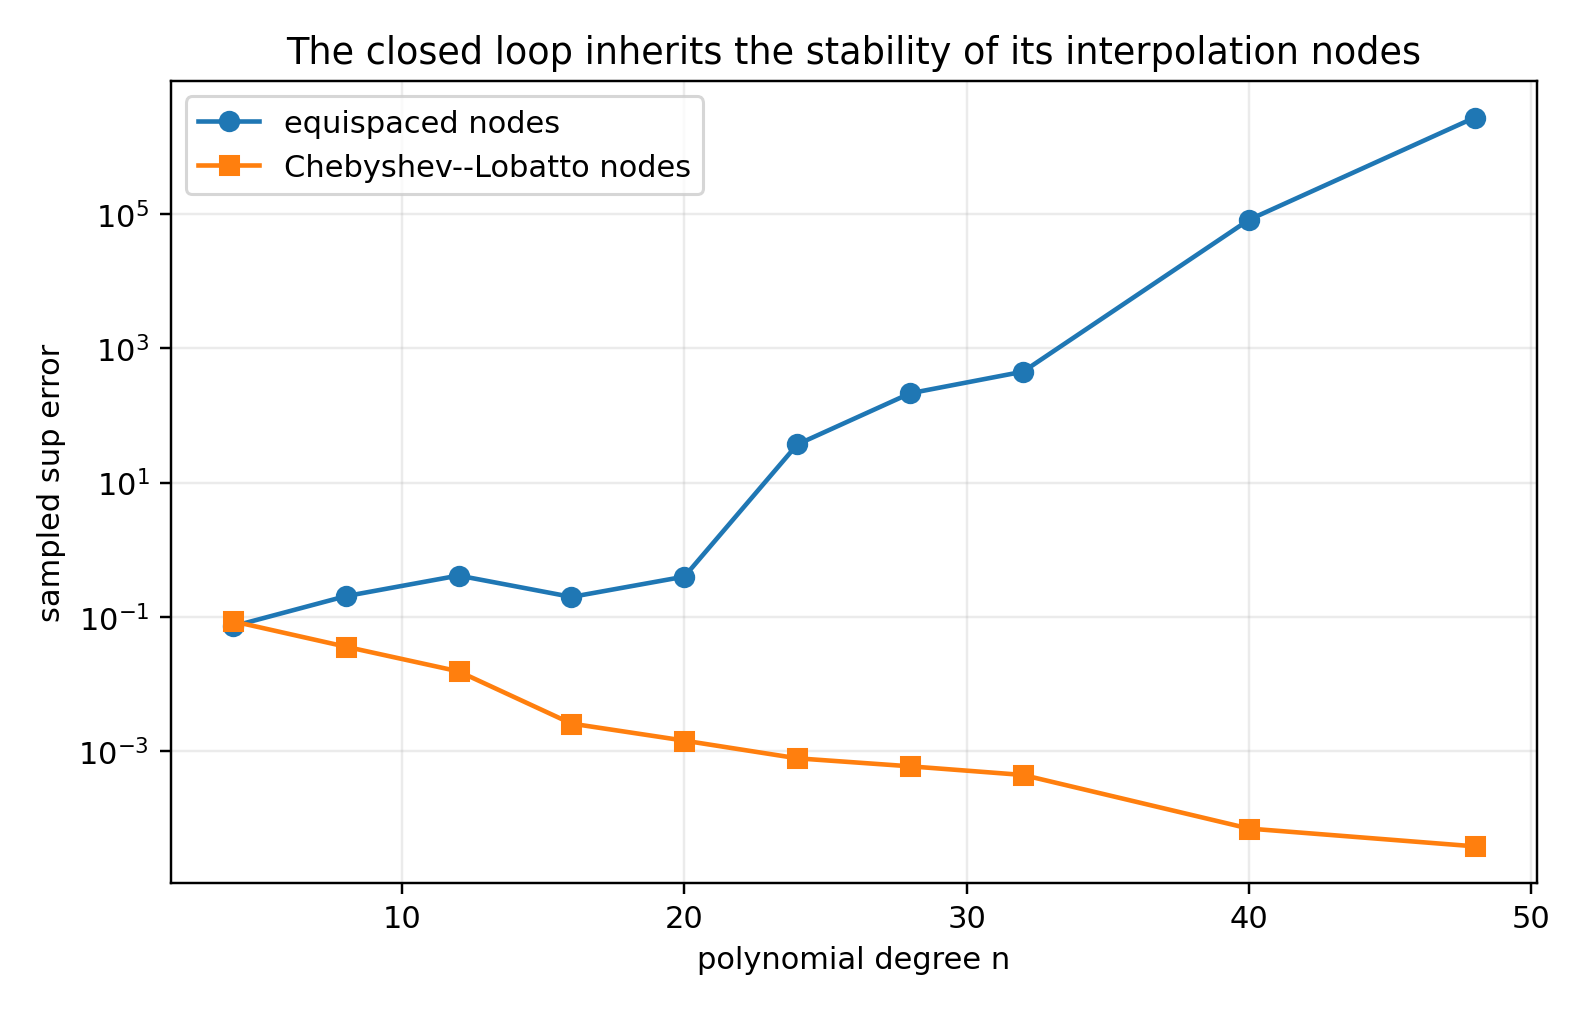
\includegraphics[width=0.92\textwidth]{interpolation_stability.png}
\caption{Sampled sup errors for a finite-convolution approximation of $u$.
The closed loop has exactly these interpolation errors on $[-1,1]$.
Chebyshev--Lobatto nodes converge, whereas equispaced nodes exhibit Runge
growth.}
\label{fig:stability}
\end{figure}

\section{Chebyshev closure and a genuinely convergent self-series}
\label{sec:chebyshev}

\subsection{Superalgebraic convergence}

Let $I_n^{\mathrm{CL}}$ denote interpolation at the $n+1$
Chebyshev--Lobatto nodes.  Since $u\in C^\infty[-1,1]$, its best polynomial
approximation error satisfies
\begin{equation}
 E_n(u):=\inf_{p\in\Pi_n}\Norm{u-p}_\infty
 =\BigO(n^{-m})
 \qquad\text{for every }m>0.
 \label{eq:best-super}
\end{equation}
The Chebyshev--Lobatto Lebesgue constant is $\BigO(\log n)$, so Lebesgue's
lemma gives \cite{BerrutTrefethen2004,Trefethen2013,RepresentationRepo}
\begin{equation}
 \Norm{u-I_n^{\mathrm{CL}}u}_\infty
 \le(1+\Lambda_n)E_n(u)=\BigO(n^{-p})
 \qquad\text{for every }p>0.
 \label{eq:cheb-super}
\end{equation}

\begin{theorem}[Uniform superalgebraic closed loop]
\label{thm:cheb-loop}
Let $x_j=\cos(j\pi/n)$ and let $b_{j,r}^{\mathrm{CL}}$ be the exact cardinal
coefficients from \cref{thm:cardinal-synth}.  Then
\begin{equation}
 u(x)=\lim_{n\to\infty}\frac1{2^n}\sum_{r=0}^{n+1}
 \left(\sum_{j=0}^nu(x_j)b_{j,r}^{\mathrm{CL}}\right)
 u\!\left(\frac{x-c_{n,r}}{2^{n+1}}\right)
 \label{eq:cheb-loop-limit}
\end{equation}
uniformly for $x\in[-1,1]$, and the function error is
$\BigO(n^{-p})$ for every $p>0$.
\end{theorem}

\begin{proof}
The finite sum in \eqref{eq:cheb-loop-limit} equals
$I_n^{\mathrm{CL}}u$ by \cref{thm:finite-loop}.  The convergence and rate are
therefore exactly \eqref{eq:cheb-super}.
\end{proof}

\subsection{Why the rate cannot be geometric}

The Fabius function is a nowhere analytic $C^\infty$ function, and so is the
corresponding up-function on its interior pieces.  If a fixed $\rho>1$ and
$C>0$ satisfied
\[
 \Norm{u-I_n^{\mathrm{CL}}u}_\infty\le C\rho^{-n},
\]
then the best approximation errors would obey the same bound.  Bernstein's
converse theorem would imply analytic continuation to a Bernstein ellipse,
contradicting nowhere analyticity.

\begin{corollary}[Exact root rate]
\label{cor:root-rate}
For the Chebyshev closed loop,
\begin{equation}
 \limsup_{n\to\infty}
 \Norm{u-I_n^{\mathrm{CL}}u}_\infty^{1/n}=1.
 \label{eq:root-rate}
\end{equation}
Thus convergence is faster than every algebraic power but slower than every
fixed geometric rate.
\end{corollary}

\begin{proof}
Superalgebraic convergence gives a limsup at most $1$.  If the limsup were
strictly below $1$, a geometric upper bound would hold for all sufficiently
large $n$, contradicting the preceding argument.
\end{proof}

\subsection{A telescoping up-series}

Set $N_m=2^m$ and
\[
 J_m=I_{N_m}^{\mathrm{CL}}u,
 \qquad J_{-1}=0,
 \qquad Q_m=J_m-J_{m-1}.
\]
Then
\begin{equation}
 u=\sum_{m=0}^{\infty}Q_m
 \label{eq:telescoping-poly}
\end{equation}
uniformly.  In fact, for every $p>0$,
\[
 \Norm{Q_m}_\infty
 \le\Norm{u-J_m}_\infty+\Norm{u-J_{m-1}}_\infty
 =\BigO(2^{-pm}),
\]
so the series is absolutely convergent in the Banach space $C[-1,1]$.
Synthesizing each $Q_m\in\Pi_{N_m}$ yields
\begin{equation}
 Q_m(x)=\frac1{2^{N_m}}
 \sum_{r=0}^{N_m+1}d_{m,r}
 u\!\left(\frac{x-c_{N_m,r}}{2^{N_m+1}}\right).
 \label{eq:block-up}
\end{equation}

\begin{theorem}[Genuine convergent self-series]
\label{thm:self-series}
The up-function admits the uniformly and absolutely convergent function-space
series
\begin{equation}
 \boxed{
 u(x)=\sum_{m=0}^{\infty}\frac1{2^{N_m}}
 \sum_{r=0}^{N_m+1}d_{m,r}
 u\!\left(\frac{x-c_{N_m,r}}{2^{N_m+1}}\right),
 \qquad N_m=2^m.}
 \label{eq:self-series}
\end{equation}
Absolute convergence here means
$\sum_m\Norm{Q_m}_\infty<\infty$; it does not imply absolute convergence of
the scalar atom amplitudes.
\end{theorem}

\begin{proof}
Equation \eqref{eq:telescoping-poly} is a telescoping identity whose partial
sums are $J_m$.  The superalgebraic estimate proves absolute convergence in
$C[-1,1]$.  Apply exact endpoint synthesis to each polynomial $Q_m$ to obtain
\eqref{eq:block-up}; substitution into \eqref{eq:telescoping-poly} proves
\eqref{eq:self-series}.
\end{proof}

\section{Endpoint conditioning and the Lambert-scale barrier}
\label{sec:conditioning}

We now prove that the exact endpoint representation is intrinsically
ill-conditioned in coefficient norm, irrespective of interpolation nodes.

\subsection{A universal amplitude lower bound}

Write the raw-amplitude form of \eqref{eq:cardinal-up} as
\begin{equation}
 P(x)=\sum_{r=0}^{n+1}a_r
 u\!\left(\frac{x-c_{n,r}}{2^{n+1}}\right),
 \qquad a_r=2^{-n}b_r.
 \label{eq:raw-form}
\end{equation}
Let
\begin{equation}
 \delta_n=\frac{n+2}{2^n}.
 \label{eq:delta}
\end{equation}
For every $x\in[-1,1]$ and every endpoint centre $c_{n,r}$, a direct range
calculation gives
\begin{equation}
 -1\le\frac{x-c_{n,r}}{2^{n+1}}\le-1+\delta_n.
 \label{eq:argument-range}
\end{equation}
Since $u(-1+s)=F(s)$ and $F$ is increasing,
\begin{equation}
 0\le u\!\left(\frac{x-c_{n,r}}{2^{n+1}}\right)
 \le F(\delta_n).
 \label{eq:atom-bound}
\end{equation}

\begin{theorem}[Endpoint amplitude barrier]
\label{thm:amplitude-barrier}
Every representation \eqref{eq:raw-form} of a polynomial $P\in\Pi_n$ in
the endpoint basis satisfies
\begin{equation}
 \boxed{
 \Norm{a}_1\ge\frac{\Norm{P}_\infty}{F(\delta_n)},
 \qquad
 \Norm{b}_1\ge\frac{2^n\Norm{P}_\infty}{F(\delta_n)}.}
 \label{eq:amplitude-bound}
\end{equation}
In particular, for every Lagrange cardinal polynomial,
\begin{equation}
 \Norm{a_j}_1\ge\frac1{F(\delta_n)}.
 \label{eq:cardinal-lower}
\end{equation}
\end{theorem}

\begin{proof}
From \eqref{eq:atom-bound}, for every $x\in[-1,1]$,
\[
 \AbsoluteValue{P(x)}
 \le\sum_r\AbsoluteValue{a_r}
 u\!\left(\frac{x-c_{n,r}}{2^{n+1}}\right)
 \le F(\delta_n)\Norm{a}_1.
\]
Take the supremum in $x$.  Since $b=2^na$, the second inequality follows.
A cardinal polynomial takes the value $1$ at its own node, so its sup norm is
at least $1$.
\end{proof}

\subsection{Quadratic-exponential growth}

Write
\begin{equation}
 \delta_n=2^{-t_n},
 \qquad t_n=n-\log_2(n+2).
 \label{eq:tn}
\end{equation}
Combining \eqref{eq:cardinal-lower} with the dyadic law
\eqref{eq:dyadic-law} yields the main asymptotic consequence.

\begin{corollary}[Lambert-scale coefficient growth]
\label{cor:quadratic-growth}
For every sequence of endpoint representations of normalized polynomials
$P_n\in\Pi_n$ with $\Norm{P_n}_\infty\ge1$,
\begin{equation}
 \log\Norm{a^{(n)}}_1
 \ge\left(\frac{\log2}{2}+o(1)\right)t_n^2,
 \label{eq:t-growth}
\end{equation}
and therefore
\begin{equation}
 \boxed{
 \liminf_{n\to\infty}\frac1{n^2}\log\Norm{a^{(n)}}_1
 \ge\frac{\log2}{2}.}
 \label{eq:n2-growth}
\end{equation}
The same leading lower bound holds for $\Norm{b^{(n)}}_1$.
\end{corollary}

\begin{proof}
Theorem \ref{thm:amplitude-barrier} gives
$\log\Norm{a^{(n)}}_1\ge-\log F(2^{-t_n})=g(t_n)$.
Since $t_n\to\infty$, \eqref{eq:dyadic-law} proves
\eqref{eq:t-growth}.  Finally $t_n/n\to1$, giving
\eqref{eq:n2-growth}.  Multiplication by $2^n$ changes the logarithm by only
$n\log2=o(n^2)$.
\end{proof}

\subsection{Stable output versus unstable internal coordinates}

For Chebyshev nodes, the function-space interpolation operator has norm
$\BigO(\log n)$ and converges superalgebraically on $u$.  Nevertheless, every
individual cardinal column of the endpoint synthesis matrix has
$\ell^1$ norm at least
\[
 \exp\!\left(\left(\frac{\log2}{2}+o(1)\right)n^2\right).
\]
Thus the map from nodal data to raw endpoint amplitudes is vastly more
ill-conditioned than the map from nodal data to the represented function.
This is exact cancellation, not approximation error.

A degree-$4$ numerical loop illustrates the phenomenon.  The grouped raw
amplitudes have $\ell^1$ norm about $1.16\times10^6$, although the represented
polynomial has size about $1$.  The finite-convolution evaluation leaves a
$2.3\times10^{-4}$ discrepancy between the two visually coincident
polynomial curves; the exact symbolic identity has zero discrepancy.

\begin{figure}[htbp]
\centering
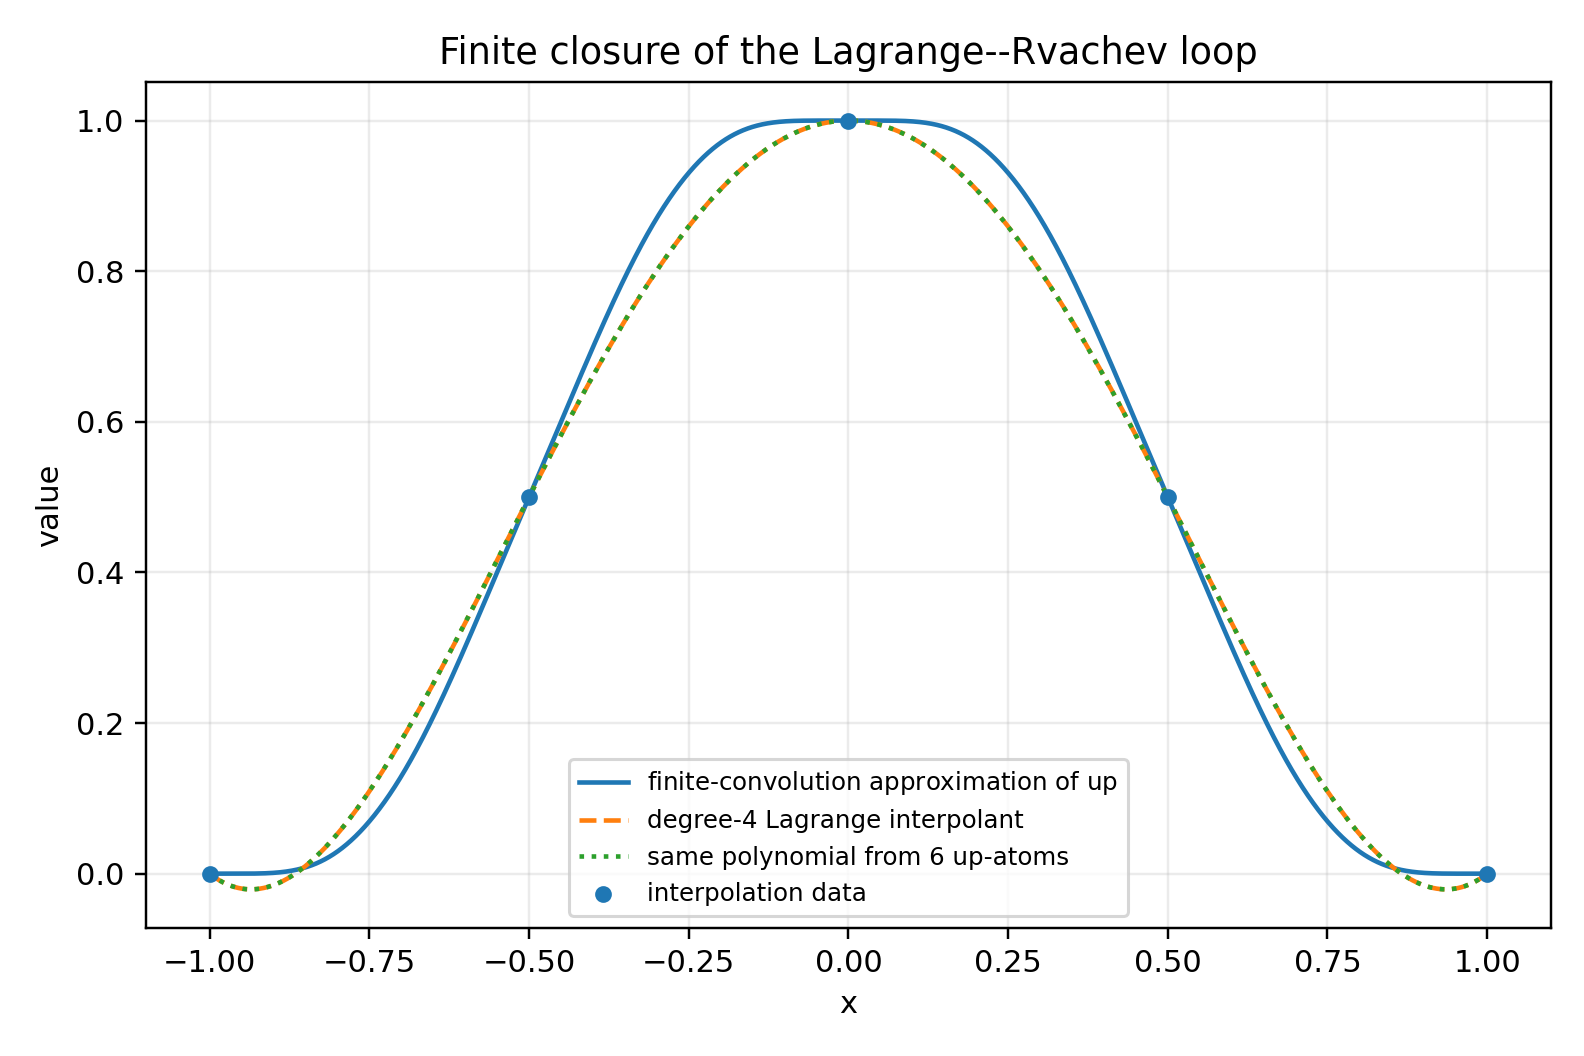
\includegraphics[width=0.92\textwidth]{finite_loop_demo.png}
\caption{Finite degree-$4$ closure.  The dashed Lagrange interpolant and dotted
six-atom reconstruction are mathematically identical.  Their small visible
numerical discrepancy is caused by cancellation among amplitudes whose total
variation is about $1.16\times10^6$.}
\label{fig:finite-loop}
\end{figure}

\subsection{Exact coefficient data}

The reproducibility script computes equispaced cardinal matrices exactly over
$\mathbb Q$.  Let
\[
 L_n=\max_{0\le j\le n}\sum_{r=0}^{n+1}
 \AbsoluteValue{2^{-n}b_{j,r}}.
\]
Selected exact-arithmetic results are shown below.

\begin{center}
\begin{tabular}{rrrr}
\toprule
$n$ & $\log_{10}L_n$ & endpoint-law proxy & $L_n$ (scientific)\\
\midrule
1 & 0.4771 & 0.0515 & $3.00\times10^0$\\
2 & 1.9401 & 0.0000 & $8.71\times10^1$\\
3 & 4.0171 & 0.0692 & $1.04\times10^4$\\
4 & 6.5522 & 0.3014 & $3.57\times10^6$\\
5 & 9.4620 & 0.7236 & $2.90\times10^9$\\
6 & 12.7880 & 1.3546 & $6.14\times10^{12}$\\
8 & 20.5134 & 3.2939 & $3.26\times10^{20}$\\
10 & 29.6674 & 6.1941 & $4.65\times10^{29}$\\
12 & 40.2033 & 10.1025 & $1.60\times10^{40}$\\
13 & 45.9670 & 12.4453 & $9.27\times10^{45}$\\
\bottomrule
\end{tabular}
\end{center}

The ``endpoint-law proxy'' is
$\frac{\log2}{2\log10}t_n^2$ and records only the rigorous leading lower-bound
scale.  The large gap at moderate $n$ reflects substantial lower-order terms,
node conditioning, and non-sharpness of replacing all atom values by the
single maximum $F(\delta_n)$.

\begin{figure}[htbp]
\centering
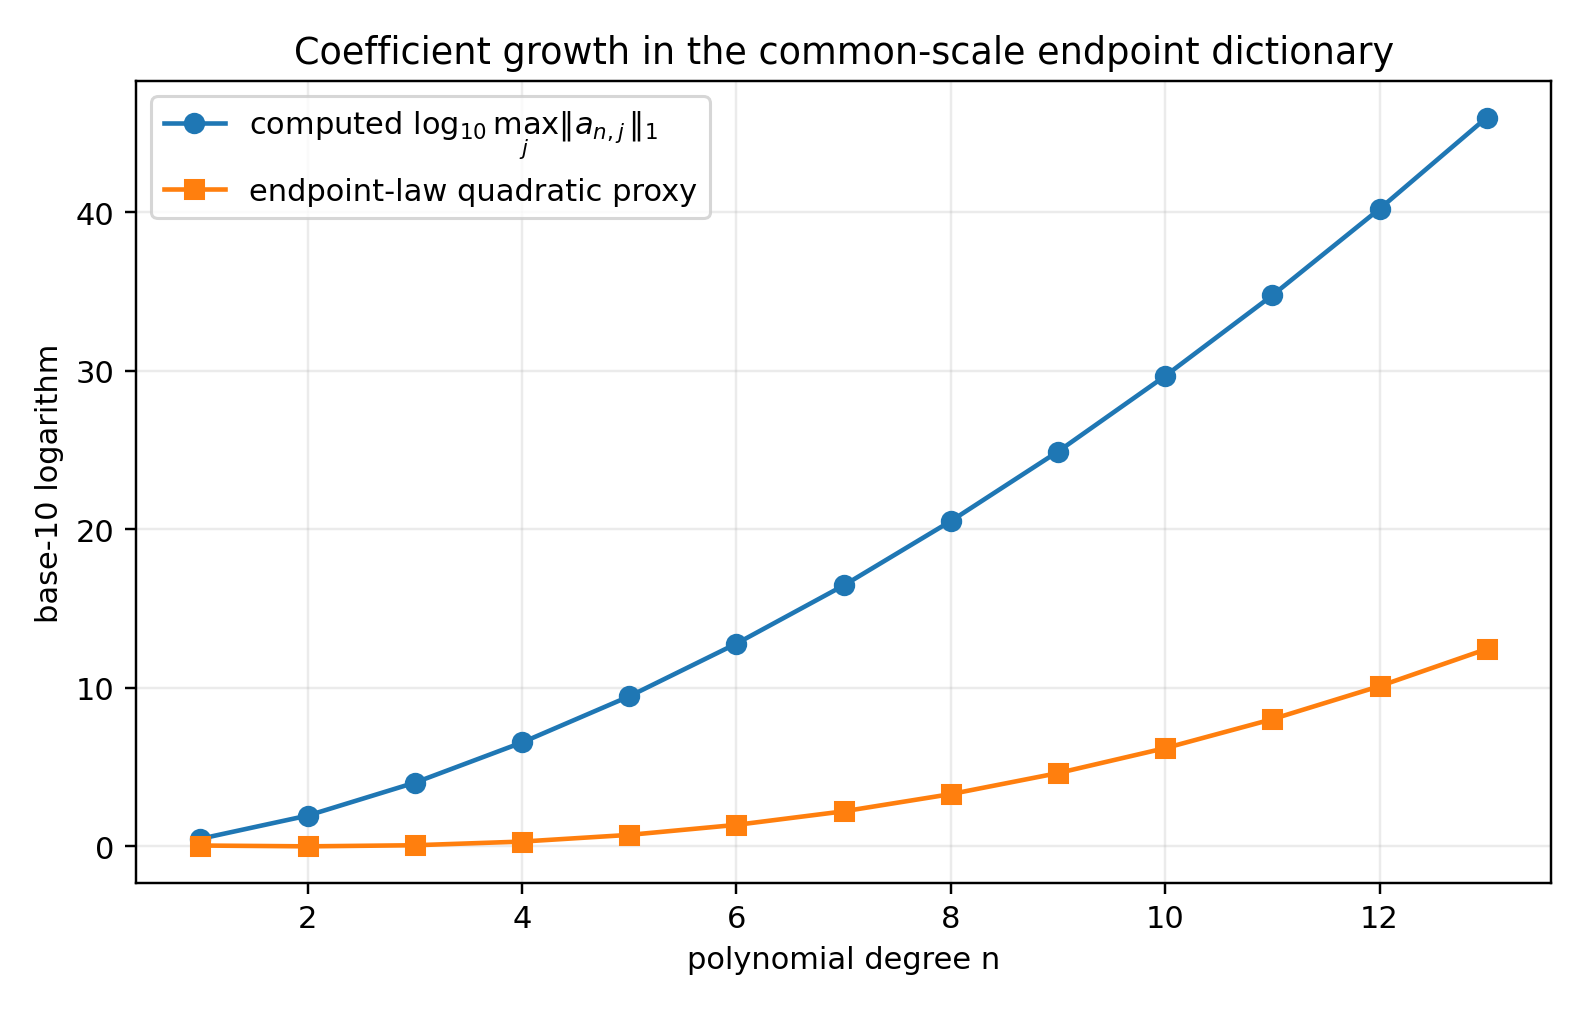
\includegraphics[width=0.92\textwidth]{coefficient_growth.png}
\caption{Exact rational coefficient norms through degree $13$, compared with
the leading quadratic endpoint-law proxy.  Both curves are quadratic in
scale; the computed cardinal coefficients contain large lower-order
contributions.}
\label{fig:growth}
\end{figure}

\section{Numerical experiments and reproducibility}
\label{sec:numerics}

\subsection{Exact arithmetic component}

The accompanying script \path{experiments.py} performs the following exact
steps with SymPy rationals:

\begin{enumerate}
\item constructs the truncated logarithm \eqref{eq:logH} and exponentiates it
through degree $n$;
\item computes only the first $n+2$ coefficients of $A_n(z)$, truncating every
convolution;
\item builds each rational Lagrange cardinal polynomial;
\item applies $H_n(D)$, samples at $r-n/2$, and solves
\eqref{eq:triangular};
\item verifies the degree-$0$, degree-$1$, and degree-$2$ monomial examples;
\item verifies the restricted Thue--Morse certificate
$\lambda_n^TB_X=0$ through degree $13$;
\item writes exact coefficient norms to \path{coefficient_growth.csv}.
\end{enumerate}

\subsection{Finite-convolution approximation of \texorpdfstring{$u$}{u}}

For plotting only, the script uses the probability representation
$X=\sum2^{-j}U_j$.  After the first summand, the density is exactly constant
on $[-1/2,1/2]$.  Convolution with the next uniform box of half-width $a$ is
implemented by
\begin{equation}
 f_{\mathrm{new}}(x)=\frac{F_{\mathrm{old}}(x+a)-F_{\mathrm{old}}(x-a)}{2a},
 \label{eq:box-average}
\end{equation}
where $F_{\mathrm{old}}$ is a numerically integrated CDF.  Twenty boxes on a
$2^{18}$-interval grid give mass $1$ and $u(0)\approx0.99999237$.

\subsection{Interpolation diagnostics}

\begin{center}
\begin{tabular}{rrr}
\toprule
$n$ & equispaced sampled error & Chebyshev--Lobatto sampled error\\
\midrule
4  & $7.20\times10^{-2}$ & $8.54\times10^{-2}$\\
8  & $2.02\times10^{-1}$ & $3.58\times10^{-2}$\\
12 & $4.11\times10^{-1}$ & $1.53\times10^{-2}$\\
16 & $1.97\times10^{-1}$ & $2.55\times10^{-3}$\\
20 & $3.96\times10^{-1}$ & $1.42\times10^{-3}$\\
24 & $3.70\times10^{1}$  & $7.74\times10^{-4}$\\
28 & $2.14\times10^{2}$  & $5.88\times10^{-4}$\\
32 & $4.50\times10^{2}$  & $4.37\times10^{-4}$\\
40 & $8.24\times10^{4}$  & $6.95\times10^{-5}$\\
48 & $2.76\times10^{6}$  & $3.77\times10^{-5}$\\
\bottomrule
\end{tabular}
\end{center}

The exact theory does not depend on these values.  Their role is to show that
the finite loop behaves exactly as the interpolation theorem predicts and to
expose the numerical effect of coefficient cancellation.

\section{Connections with the surrounding Fabius--Rvachev theory}
\label{sec:connections}

\subsection{Thue--Morse and the \texorpdfstring{$q$}{q}-integer annihilator}

The polynomial
\[
 A_n(z)=\prod_{m=1}^n[2^m]_z
\]
is simultaneously a reproduction filter, a $q$-integer product, and the
source of the Thue--Morse polynomiality certificate.  The factorization
\[
 A_n(z)(z-1)^{n+1}
 =(-1)^{n+1}(1-z)\prod_{m=0}^n(1-z^{2^m})
\]
exhibits the finite Thue--Morse product.  In the loop, this same object has
three roles:

\begin{enumerate}
\item its low coefficients form the Toeplitz deconvolution in
\eqref{eq:triangular};
\item its value $A_n(1)=2^{n(n+1)/2}$ sets the natural arithmetic scale;
\item its signed coefficient functional supplies the final row that makes the
sampling matrix invertible.
\end{enumerate}

Thus the Thue--Morse sequence does not enter only as a decorative identity;
it is the exact algebraic separator between the polynomial hyperplane and the
single local defect mode.

\subsection{Bell and Bernoulli polynomials}

The inverse moment transform $M_u(D)^{-1}$ and the scale correction
$(D/[2\sinh(D/2)])^n$ combine into $H_n(D)$.  Their logarithms add, so
cumulants linearize the synthesis problem.  Complete Bell polynomials then
convert cumulants to ordinary differential coefficients \cite{Comtet}.  This is precisely
why the cardinal formula \eqref{eq:explicit-b} is finite: the degree-$n$
polynomial kills every derivative above $n$.

The same mechanism can be expressed in the repository's up-Appell family.
If $\widetilde G_m(y)=M_u(D)^{-1}y^m$, then $H_n(D)$ is obtained by composing
that Appell inverse with the $n$th power of the centered-box deconvolution.
The cardinal synthesis coefficients can therefore also be expanded in an
Appell basis rather than monomials.

\subsection{Infinite sinc products and Strang--Fix reproduction}

The Fourier zeros of
$\widehat u(\xi)=\prod_j\SincRad(\xi/2^j)$ have dyadic multiplicities.  At scale
$2^n$, nonzero lattice frequencies have enough zero multiplicity to reproduce
all polynomials through degree $n$.  This is the spectral reason the common
scale is $2^n$ and the shift family has approximation order $n+1$
\cite{StrangFix,deBoorRon,UpSynthesisRepo}.  The one
extra local dimension is not a failure of Strang--Fix reproduction; it is the
finite-cell alias defect isolated by $E_n$.

\subsection{Lambert \texorpdfstring{$W$}{W} and numerical conditioning}

The lower branch $W_{-1}$ describes the saddle scale at the flat endpoint of
$F$ \cite{Corless1996,PrimaryRepo}.  In the loop, the relevant endpoint argument is
$\delta_n=(n+2)2^{-n}$.  Consequently, the exact large-amplitude cancellation
is governed by the same Lambert phase that controls small-argument Fabius
asymptotics.  This is a direct bridge from asymptotic analysis to numerical
linear algebra: the smallest atom magnitude bounds the inverse coordinate
map.

\subsection{Lagrange residual moments and the ghost}

For arbitrary nodes, the residual of degree $n+1$ is the nodal polynomial
$\omega_X$.  For geometric nodes, higher residual moments are complete
homogeneous symmetric polynomials and simplify to Gaussian-binomial
expressions.  The ghost identity
\[
 G_{n,X}=\omega_X+(I-I_X)E_n
\]
shows how those classical interpolation residuals are modified by the
canonical Rvachev defect.  The polynomial and Fourier parts are therefore not
separate phenomena; together they form the unique null mode of atom sampling.

\subsection{Inverse Fabius and adaptive sampling}

The endpoint coefficient barrier depends on $F(\delta_n)$.  Any sharper
asymptotic expansion for the inverse Fabius function immediately translates
into a sharper statement about the degree at which a prescribed coefficient
budget becomes impossible.  Conversely, measured coefficient growth in
carefully normalized dictionaries provides indirect numerical data about the
endpoint scale.  This duality suggests using inverse-Fabius asymptotics to
choose adaptive degree and cell size in multi-cell synthesis.

\section{Frontier conjectures and open problems}
\label{sec:conjectures}

The following statements are plausible consequences of the exact framework
and numerical evidence, but they are not proved here.

\begin{conjecture}[Sharp Lambert--phase amplitude asymptotic]
\label{conj:sharp-lambert}
For normalized endpoint cardinal columns in a regular node family,
\begin{equation}
 \log\Norm{a_{n,j}}_1
 =-\log F((n+2)2^{-n})+\Gamma_{X,j}(n)+o(1),
 \label{eq:sharp-lambert-conj}
\end{equation}
where $\Gamma_{X,j}(n)$ has at most order $n\log n$ and admits a decomposition
into a smooth part plus a bounded nonconstant periodic function of the lower
Lambert phase.  After subtraction of the full known endpoint expansion, the
normalized residual should be precompact and oscillatory rather than
convergent.
\end{conjecture}

\begin{conjecture}[Universality of the quadratic constant]
\label{conj:universal-half}
Among all consecutive common-scale endpoint blocks at the sharp ratio $2^n$,
translation of the block can alter lower-order conditioning but cannot reduce
the leading constant $\log2/2$ in the logarithmic coefficient growth required
to represent unit-size degree-$n$ polynomials on one cell.
\end{conjecture}

\begin{conjecture}[Central-basis improvement]
\label{conj:central}
The unresolved central consecutive $(n+2)$-atom basis is nonsingular for every
$n$.  After natural diagonal scaling by endpoint values and factorial/Appell
weights, its condition number grows strictly more slowly than that of the
right-endpoint basis, perhaps as $\exp(\BigO(n\log n))$ rather than
$\exp(\Theta(n^2))$.
\end{conjecture}

\begin{conjecture}[Ghost singular-vector principle]
\label{conj:ghost-sv}
For standard node families, the coefficient vector of
$G_{n,X}=D_n-I_XD_n$ converges after diagonal normalization to the extremal
right singular vector of the atom-sampling matrix.  Its left singular partner
is asymptotically the restricted Thue--Morse certificate.
\end{conjecture}

\begin{conjecture}[Basic hypergeometric compression]
\label{conj:q-hyper}
For geometric nodes $\theta_j=q^j$, the finite formula of
\cref{prop:q-bell} can be resummed into a terminating basic hypergeometric
expression in $j$ and $r$, with the Bell multiplier appearing as a finite
$q$-difference deformation of the up-Appell family.
\end{conjecture}

\begin{question}[Arithmetic valuations]
For dyadic rational nodes, how large are the odd denominator and $2$-adic
valuation of $b_{j,r}$?  Real norms grow quadratically-exponentially, but the
exact rational data suggest that the $2$-adic structure may remain governed
by short Thue--Morse recurrences.  Can one obtain exact valuation formulas?
\end{question}

\begin{question}[Optimal total variation]
The endpoint basis is unique, so its amplitude norm is fixed.  If arbitrary
centres and scales are allowed, what is the minimum total variation
\[
 \inf\left\{\sum_s\AbsoluteValue{a_s}:P(x)=\sum_sa_su((x-c_s)/\sigma_s)
 \text{ on }[-1,1]\right\}?
\]
Can positivity, sign-change counts, or moment duality produce scale-independent
lower bounds?  Lagrange cardinals that change sign cannot admit a positive
representation.
\end{question}

\begin{question}[Multi-cell balance]
On a partition into $J$ cells, the physical atom scale and atom count can be
traded against each other.  What choice of $J=J(n,\epsilon)$ minimizes total
work under simultaneous approximation-error and coefficient-budget
constraints?  The answer should couple Chebyshev $hp$ approximation with
inverse-Fabius endpoint asymptotics.
\end{question}

\section{Algorithms}
\label{sec:algorithms}

\begin{algorithm}[Exact synthesis of one Lagrange cardinal]
\label{alg:cardinal}
Input: degree $n$, distinct rational nodes $x_0,\ldots,x_n$, and index $j$.

\begin{enumerate}[label=\arabic*.]
\item Set $\theta_i=(x_i+1)/2$ and form
$P_{n,j}(t)=\prod_{i\ne j}(t-\theta_i)/(\theta_j-\theta_i)$.
\item Construct $\log H_n(z)$ from \eqref{eq:logH}, truncate at degree $n$,
and exponentiate formally.
\item Compute $G=H_n(D)P_{n,j}$.
\item Form only $a_{n,0},\ldots,a_{n,n+1}$ by truncated convolution of the
blocks $[2^m]_z$.
\item For $r=0,\ldots,n+1$, compute
$g_r=A_n(1)G(r-n/2)$.
\item Solve
$b_r=g_r-\sum_{s<r}a_{n,r-s}b_s$.
\item Return centres $c_{n,r}$ from \eqref{eq:centers-x} and amplitudes
$2^{-n}b_r$.
\end{enumerate}
\end{algorithm}

\begin{algorithm}[Closed loop for one data vector]
\label{alg:loop}
Input: nodes $x_j$ and data $y_j=f(x_j)$.

\begin{enumerate}[label=\arabic*.]
\item Construct the interpolating polynomial $p_X$ in a numerically stable
basis (barycentric, Newton, or Chebyshev).
\item Convert $p_X((2t-1))$ to a polynomial in $t$ only when exact endpoint
coefficients are required.
\item Apply the degree-$n$ synthesis algorithm once to $p_X$.
\item Evaluate the $n+2$ grouped atoms.  Use extended precision or compensated
summation because the amplitude total variation can be enormous.
\end{enumerate}
\end{algorithm}

\begin{algorithm}[Stable convergent loop]
\label{alg:stable}
For approximation of $u$ rather than symbolic identity:

\begin{enumerate}[label=\arabic*.]
\item use Chebyshev--Lobatto nodes, not a single global equispaced grid;
\item choose $n$ from a Chebyshev coefficient tail or an a posteriori error
estimate;
\item keep the polynomial representation for numerical evaluation whenever
possible;
\item use the up-synthesis as an exact symbolic certificate, a compact smooth
extension, or a multiscale building block;
\item if atom evaluation is unavoidable, use high precision predicted from
$-\log F((n+2)2^{-n})$.
\end{enumerate}
\end{algorithm}

\section{Formalization roadmap}
\label{sec:formalization}

The new results are well suited to incremental Lean formalization because the
deep analytic ingredients are already represented in the repository.

\begin{enumerate}
\item Define the affine node transport and prove
$P_{n,j}(t)=\ell_{n,j}(2t-1)$.
\item Package the endpoint synthesis theorem as a linear equivalence between
$\Pi_n$ and the kernel of the certificate row.
\item Define $B_X$ by applying this equivalence to the finite Lagrange basis and
prove $\Phi_XB_X=I$.
\item Prove invertibility of $M_X$ by the polynomial zero argument in
\cref{thm:defect-completed}.
\item Formalize the rank-one projector using finite-dimensional linear
algebra.
\item Introduce $D_n$ and prove the ghost identity from
$t^{n+1}-I_Xt^{n+1}=\omega_X$.
\item Prove the endpoint amplitude bound from monotonicity of $F$ and the
explicit argument interval.
\item Combine with the already formalized or separately formalizable dyadic
endpoint law to obtain the $n^2$ lower bound.
\end{enumerate}

The only portion requiring substantial approximation-theory infrastructure is
the Chebyshev convergence theorem.  The finite algebraic loop and coefficient
barrier are otherwise elementary consequences of existing exact objects.

\section{Conclusions}

The requested loop can be closed exactly, but the result has more structure
than a formal substitution suggests.

First, every degree-$n$ Lagrange cardinal on $[-1,1]$ belongs to one common
$n+2$-atom Rvachev dictionary.  Its amplitudes are explicit combinations of
node symmetric functions, Bernoulli numbers, complete Bell polynomials, and a
$q$-integer Toeplitz inverse.  The representation is finite and exact.

Second, substituting those formulas into a Lagrange interpolant does not
create a large atom set: the double sum collapses to $n+2$ atoms.  At the
matrix level, cardinal synthesis is a right inverse of atom sampling.  The
Thue--Morse defect row supplies the unique missing equation, and the resulting
loop is a rank-one projection.  Its null mode is the canonical defect minus
its Lagrange interpolant, equivalently the nodal polynomial plus a universal
periodic correction.

Third, finite closure and asymptotic convergence are different questions.
Equispaced dyadic interpolation remains vulnerable to Runge divergence.
Chebyshev--Lobatto interpolation yields a superalgebraically convergent loop
and a genuine telescoping self-series, but no geometric rate is possible for
the nowhere analytic up-function.

Finally, the endpoint basis has an unavoidable numerical price.  Its atoms
are evaluated at the flat edge of $u$, forcing raw amplitude norms of at least
$\exp((\log2/2+o(1))n^2)$.  This converts the Lambert-$W$ endpoint asymptotics
of the Fabius function into a sharp qualitative statement about coordinate
conditioning.  The most promising next step is therefore not merely to push
degree higher, but to optimize the dictionary phase, scale, and cell
partition while preserving the exact Thue--Morse/Appell algebra.

\appendix

\section{Detailed proof of the elementary-symmetric derivative identity}

Let
\[
 P(t)=w\prod_{i=1}^n(t-\beta_i).
\]
For an auxiliary variable $h$,
\[
 P(y+h)=w\prod_{i=1}^n((y-\beta_i)+h)
 =w\sum_{q=0}^n e_{n-q}(y-\beta_1,\ldots,y-\beta_n)h^q.
\]
Taylor's formula also gives
\[
 P(y+h)=\sum_{q=0}^n\frac{P^{(q)}(y)}{q!}h^q.
\]
Equating coefficients proves \eqref{eq:derivative-elementary}.  Substitution
into \eqref{eq:HDP} proves \eqref{eq:G-cardinal} without any appeal to a
symbolic algebra system.

\section{Proof of the geometric excluded-variable identity}

Let $E_s=e_s(1,q,\ldots,q^n)$ and
$E_s^{(j)}=e_s(1,q,\ldots,\widehat{q^j},\ldots,q^n)$.  Splitting terms by
whether they use $q^j$ gives
\[
 E_s=E_s^{(j)}+q^jE_{s-1}^{(j)}.
\]
Iterating,
\[
 E_s^{(j)}=E_s-q^jE_{s-1}+q^{2j}E_{s-2}-\cdots+(-1)^sq^{sj}E_0.
\]
The finite $q$-binomial theorem gives
$E_r=q^{\binom r2}\GaussianBinomial{n+1}{r}{q}$, proving
\eqref{eq:q-excluded-e}.

\section{Exact low-degree regression identities}

The implementation checks the following imported monomial syntheses in the
$t$ coordinate:
\begin{align*}
1&=u(t)+u(t-1),\\
t&=-\frac12u\!\left(\frac t2\right)
  +u\!\left(\frac{t-1}{2}\right)
  +\frac12u\!\left(\frac{t-2}{2}\right),\\
t^2&=\frac{13}{9}u\!\left(\frac{t-1}{4}\right)
 -\frac{31}{9}u\!\left(\frac{t-2}{4}\right)
 +\frac{49}{9}u\!\left(\frac{t-3}{4}\right)
 +\frac{5}{9}u\!\left(\frac{t-4}{4}\right).
\end{align*}
These identities are used only as regression tests; the general algorithm is
not inferred from them.

\section{Reproducibility files}

The archive accompanying this report contains:

\begin{description}[style=nextline,leftmargin=2.2em]
\item[\path{Lagrange_Rvachev_Loop.tex}]
The complete LaTeX source.
\item[\path{Lagrange_Rvachev_Loop.pdf}]
The compiled report.
\item[\path{experiments.py}]
Commented exact and numerical code.
\item[\path{coefficient_growth.csv}]
Exact-arithmetic coefficient norm data through degree $13$.
\item[\path{numerical_summary.txt}]
Plain-text numerical diagnostics.
\item[\path{coefficient_growth.png}, \path{interpolation_stability.png},
\path{finite_loop_demo.png}]
Figures used in the report.
\end{description}

\section{Repository paths audited most directly}

The repository root is
\url{https://github.com/VladimirReshetnikov/ProveIt}.  The most directly
used source paths, written relative to that root, are:

\begin{sloppypar}
\small
\begin{itemize}
\item \path{Analysis/FabiusFunction/docs/}
\item \path{Analysis/FabiusFunction/docs/Fabius_Function_and_Rvachev_Up/Fabius_Function_and_Rvachev_Up.tex}
\item \path{Analysis/FabiusFunction/docs/semi-formalized-research-frontiers/drafts/representations/Up_Polynomial_Synthesis/Up_Polynomial_Synthesis.tex}
\item \path{Analysis/FabiusFunction/docs/semi-formalized-research-frontiers/drafts/inverse-and-sampling/Dyadic_Comb_Frontiers/Dyadic_Comb_Frontiers.tex}
\item \path{Analysis/FabiusFunction/docs/semi-formalized-research-frontiers/drafts/representations/Representation_Frontiers/Representation_Frontiers.tex}
\end{itemize}
\end{sloppypar}

\begin{thebibliography}{99}

\bibitem{Fabius1966}
J.~Fabius,
\newblock A probabilistic example of a nowhere analytic $C^\infty$-function,
\newblock \emph{Zeitschrift f\"ur Wahrscheinlichkeitstheorie und Verwandte
Gebiete} \textbf{5} (1966), 173--174.

\bibitem{Rvachev1971}
V.~L.~Rvachev and V.~A.~Rvachev,
\newblock A certain finite function,
\newblock \emph{Dopovidi Akademii Nauk Ukrains'koi RSR, Series A} (1971),
705--707, 764.

\bibitem{Rvachev1990}
V.~A.~Rvachev,
\newblock Compactly supported solutions of functional-differential equations
and their applications,
\newblock \emph{Russian Mathematical Surveys} \textbf{45} (1990), no.~1,
87--120.

\bibitem{Arias1982}
J.~Arias de Reyna,
\newblock Definici\'on y estudio de una funci\'on indefinidamente diferenciable
de soporte compacto,
\newblock \emph{Revista de la Real Academia de Ciencias Exactas, F\'isicas y
Naturales de Madrid} \textbf{76} (1982), no.~1, 21--38; English translation,
arXiv:1702.05442.

\bibitem{Arias2018}
J.~Arias de Reyna,
\newblock Arithmetic of the Fabius function,
\newblock \emph{INTEGERS} \textbf{18} (2018), Article A51;
arXiv:1702.06487, version 3.

\bibitem{Haugland2016}
J.~K.~Haugland,
\newblock Evaluating the Fabius function,
\newblock arXiv:1609.07999 (2016).

\bibitem{AlloucheShallit}
J.-P.~Allouche and J.~Shallit,
\newblock \emph{Automatic Sequences: Theory, Applications, Generalizations},
\newblock Cambridge University Press, 2003.

\bibitem{Comtet}
L.~Comtet,
\newblock \emph{Advanced Combinatorics},
\newblock Reidel, 1974.

\bibitem{StrangFix}
G.~Strang and G.~Fix,
\newblock A Fourier analysis of the finite element variational method,
\newblock in \emph{Constructive Aspects of Functional Analysis}, C.I.M.E.,
1973, 793--840.

\bibitem{deBoorRon}
C.~de~Boor and A.~Ron,
\newblock Fourier analysis of the approximation power of principal
shift-invariant spaces,
\newblock \emph{Constructive Approximation} \textbf{8} (1992), 427--462.

\bibitem{Runge1901}
C.~Runge,
\newblock \"Uber empirische Funktionen und die Interpolation zwischen
\"aquidistanten Ordinaten,
\newblock \emph{Zeitschrift f\"ur Mathematik und Physik} \textbf{46} (1901),
224--243.

\bibitem{MillsSmith1992}
T.~M.~Mills and S.~J.~Smith,
\newblock The Lebesgue constant for Lagrange interpolation on equidistant
nodes,
\newblock \emph{Numerische Mathematik} \textbf{61} (1992), 111--115.

\bibitem{BerrutTrefethen2004}
J.-P.~Berrut and L.~N.~Trefethen,
\newblock Barycentric Lagrange interpolation,
\newblock \emph{SIAM Review} \textbf{46} (2004), no.~3, 501--517.

\bibitem{Trefethen2013}
L.~N.~Trefethen,
\newblock \emph{Approximation Theory and Approximation Practice},
\newblock SIAM, 2013.

\bibitem{Corless1996}
R.~M.~Corless, G.~H.~Gonnet, D.~E.~G.~Hare, D.~J.~Jeffrey, and D.~E.~Knuth,
\newblock On the Lambert $W$ function,
\newblock \emph{Advances in Computational Mathematics} \textbf{5} (1996),
329--359.

\bibitem{DLMF}
F.~W.~J.~Olver et al., eds.,
\newblock \emph{NIST Digital Library of Mathematical Functions},
\newblock \url{https://dlmf.nist.gov/}.

\bibitem{PrimaryRepo}
V.~Reshetnikov,
\newblock \emph{Fabius Function and Rvachev Up: Primary Exposition},
\newblock ProveIt repository, current source inspected 29 August 2026.

\bibitem{UpSynthesisRepo}
V.~Reshetnikov,
\newblock \emph{Exact Polynomial Synthesis by Finite Rvachev Up-Function
Dictionaries} (consolidated as \emph{Up Polynomial Synthesis}),
\newblock ProveIt repository, current source inspected 29 August 2026.

\bibitem{DyadicCombRepo}
V.~Reshetnikov,
\newblock \emph{Dyadic Comb Frontiers},
\newblock ProveIt repository, current source inspected 29 August 2026.

\bibitem{RepresentationRepo}
V.~Reshetnikov,
\newblock \emph{Representation Frontiers},
\newblock ProveIt repository, current source inspected 29 August 2026.

\end{thebibliography}

\end{document}
